\documentclass[11pt]{article}

% Change "review" to "final" to generate the final (sometimes called camera-ready) version.
% Change to "preprint" to generate a non-anonymous version with page numbers.
\usepackage[final]{acl}

% Standard package includes
\usepackage{times}
\usepackage{latexsym}

% For proper rendering and hyphenation of words containing Latin characters (including in bib files)
\usepackage[T1]{fontenc}
% For Vietnamese characters
% \usepackage[T5]{fontenc}
% See https://www.latex-project.org/help/documentation/encguide.pdf for other character sets

% This assumes your files are encoded as UTF8
\usepackage[utf8]{inputenc}

% This is not strictly necessary, and may be commented out,
% but it will improve the layout of the manuscript,
% and will typically save some space.
\usepackage{microtype}

% This is also not strictly necessary, and may be commented out.
% However, it will improve the aesthetics of text in
% the typewriter font.
\usepackage{inconsolata}

%Including images in your LaTeX document requires adding
%additional package(s)
\usepackage{graphicx}

\usepackage{amsmath}
\usepackage{booktabs}
\usepackage{xcolor}
\usepackage{float}
% If the title and author information does not fit in the area allocated, uncomment the following
%
%\setlength\titlebox{<dim>}
%
% and set <dim> to something 5cm or larger.

\newcommand{\red}[1]{\textcolor{red}{#1}}

\title{BSCodec: A Band-Split Neural Codec for High-Quality Universal Audio Reconstruction}

% Author information can be set in various styles:
% For several authors from the same institution:
% \author{Author 1 \and ... \and Author n \\
%         Address line \\ ... \\ Address line}
% if the names do not fit well on one line use
%         Author 1 \\ {\bf Author 2} \\ ... \\ {\bf Author n} \\
% For authors from different institutions:
% \author{Author 1 \\ Address line \\  ... \\ Address line
%         \And  ... \And
%         Author n \\ Address line \\ ... \\ Address line}
% To start a separate ``row'' of authors use \AND, as in
% \author{Author 1 \\ Address line \\  ... \\ Address line
%         \AND
%         Author 2 \\ Address line \\ ... \\ Address line \And
%         Author 3 \\ Address line \\ ... \\ Address line}

% \author{First Author \\
%   Affiliation / Address line 1 \\
%   Affiliation / Address line 2 \\
%   Affiliation / Address line 3 \\
%   \texttt{email@domain} \\\And
%   Second Author \\
%   Affiliation / Address line 1 \\
%   Affiliation / Address line 2 \\
%   Affiliation / Address line 3 \\
%   \texttt{email@domain} \\}

\author{
 \textbf{Haoran Wang\textsuperscript{1,2}},
 \textbf{Jiatong Shi\textsuperscript{1}},
 \textbf{Jinchuan Tian\textsuperscript{1}},
 \textbf{Bohan Li\textsuperscript{2}},
\\
 \textbf{Kai Yu\textsuperscript{2}},
 \textbf{Shinji Watanabe\textsuperscript{1}\thanks{Corresponding author.}}
\\
 \textsuperscript{1}Carnegie Mellon University~~
 \textsuperscript{2}Shanghai Jiao Tong University
\\
 % \small{
 %   \textbf{Correspondence:} \href{mailto:email@domain}{email@domain}
 % }
}

\begin{document}
\maketitle
\begin{abstract}

% While recent neural audio codecs excel at reconstructing speech at very low bitrates, their performance on general audio and music remains a significant challenge. We introduce BSCodec (Band-Split Codec), a novel architecture that achieves strong performance on music and general audio while retaining high potential for speech. Our method employs a Short-Time Fourier Transform (STFT) to decompose the input audio into independent sub-bands for parallel processing. Comprehensive objective and subjective evaluations show that BScodec surpasses existing unified neural codecs at comparable bitrates for music and audio tasks.
% Neural audio codecs have recently enabled high-fidelity reconstruction at high compression rates, especially for speech. However, speech and music exhibit fundamentally different spectral characteristics: speech energy concentrates in narrow bands around pitch harmonics (typically 80-400 Hz fundamental), while music requires faithful reproduction across the full spectrum, particularly in higher frequencies critical for timbre and texture. This spectral diversity poses a critical challenge that existing neural codecs optimized for speech suffer noticeable degradation when applied to music or general audio. We observe that uniform compression across all frequencies is suboptimal: different frequency bands have vastly different information density and perceptual importance depending on content type. To address this gap, we propose \textbf{BSCodec} (Band-Split Codec), a novel neural audio codec architecture that splits the spectral dimension into separate bands and compresses each band independently. Experimental results demonstrate that, trained on the same mixed data containing speech, music, and general audio, BSCodec achieves superior reconstruction over baselines across general audio and music, while maintaining competitive quality in the speech domain. Downstream benchmark tasks further confirm that BSCodec preserves critical audio structures, demonstrating strong potential for use in downstream applications.


% Neural audio codecs have recently enabled high-fidelity reconstruction at high compression rates, especially for speech. However, speech and non-speech audio exhibit fundamentally different spectral characteristics: speech energy concentrates in narrow bands around pitch harmonics (typically 80-400 Hz fundamental), while non-speech audio requires faithful reproduction of energy distribution across the full spectrum, particularly preserving the energy content in higher frequencies that defines timbre and texture. This spectral diversity poses a critical challenge—existing neural codecs with high compression rates, optimized for speech, suffer noticeable degradation when applied to music or sound. We observe that treating the full frequency spectrum holistically is suboptimal: different frequency bands have vastly different information density and perceptual importance depending on content type, yet full-band approaches apply uniform modeling capacity across all frequencies without accounting for these natural acoustic structures.

Neural audio codecs have recently enabled high-fidelity reconstruction at high compression rates, especially for speech. However, speech and non-speech audio exhibit fundamentally different spectral characteristics: speech energy concentrates in narrow bands around pitch harmonics (80-400 Hz), while non-speech audio requires faithful reproduction across the full spectrum, particularly preserving higher frequencies that define timbre and texture. This poses a challenge—speech-optimized neural codecs suffer degradation on music or sound. Treating the full spectrum holistically is suboptimal: frequency bands have vastly different information density and perceptual importance by content type, yet full-band approaches apply uniform capacity across frequencies without accounting for these acoustic structures. To address this gap, we propose \textbf{BSCodec} (Band-Split Codec), a novel neural audio codec architecture that splits the spectral dimension into separate bands and compresses each band independently. Experimental results demonstrate that BSCodec achieves superior reconstruction over baselines across sound and music, while maintaining competitive quality in the speech domain, when trained on the same combined dataset of speech, music and sound. Downstream benchmark tasks further confirm that BSCodec shows strong potential for use in downstream applications.\footnote{https://github.com/whr-a/espnet/tree/bscodec}
\end{abstract}
% https://anonymous.4open.science/r/espnet-2C03


% We observe that uniform compression across all frequencies is suboptimal: different frequency bands have vastly different information density and perceptual importance depending on content type.

\section{Introduction}
\label{sec:inc}
% The development of neural audio codecs has led to remarkable achievements, particularly in the domain of speech, where specialized models now deliver high-fidelity reconstruction at very low bitrates. However, progress in universal codecs—those designed to perform equally well on speech, music, and general audio—has been less pronounced. Many state-of-the-art universal models, such as DAC, are still built upon Residual Vector Quantization (RVQ). We argue that RVQ possesses an inherent limitation: it relies on a cascade of codebooks where each subsequent layer quantizes the residual error of the previous one. This residual information lacks explicit acoustic meaning, which poses a significant challenge to disentangling information across the layers and efficiently utilizing the overall codebook capacity.
% ORIGINAL:The development of neural audio codecs~\cite{zeghidour2021soundstream, kumar2023high, defossez2022high, yang2023hifi} has led to remarkable progress in audio compression and reconstruction. Building upon these advances, the speech domain has witnessed particularly significant achievements, where specialized models~\cite{ji2024wavtokenizer, defossez2024moshi, jiang2025unicodec} now deliver high-fidelity reconstruction at very low bitrates. However, progress in universal codecs—those designed to perform equally well on speech, music, and general audio—has been less pronounced. Many state-of-the-art universal models, such as DAC~\cite{kumar2023high}, are still built upon Residual Vector Quantization (RVQ). We argue that RVQ possesses an inherent limitation: it relies on a cascade of codebooks where each subsequent layer quantizes the residual error of the previous one. This residual information lacks explicit acoustic meaning, which results in a suboptimal allocation of information across the quantization hierarchy. Although RVQ demonstrates high codebook utilization, the acoustically opaque residuals prevent the model from strategically distributing perceptually meaningful information (such as pitch, timbre, and temporal structure) across different layers in a manner that best serves reconstruction quality. Furthermore, the absence of explicit acoustic structure in RVQ's residual representation poses greater challenges for the encoder-decoder architecture. Since the quantization layers do not correspond to interpretable acoustic attributes, the encoder needs to learn complex, entangled representations to prepare features for residual quantization, while the decoder must perform equally complex inverse transformations—leading to inefficient parameter usage and suboptimal reconstruction. BigCodec~\cite{xin2024bigcodec} achieves high reconstruction quality on speech at a bitrate of only 1.04 kbps by substantially increasing the number of parameters in both the encoder and decoder. This demonstrates that codebook utilization is not the sole bottleneck, and that performance can be improved through simple scaling up of the encoder-decoder architecture. Therefore, designing a codebook structure that aligns with the natural decomposition of acoustic information should enable more efficient encoder optimization and yield superior reconstruction performance under comparable codebook capacity constraints.
% The development of neural audio codecs~\cite{zeghidour2021soundstream, kumar2023high, defossez2022high, yang2023hifi} has revolutionized audio compression and reconstruction. Recent advances in the speech domain have been particularly remarkable, with specialized models~\cite{ji2024wavtokenizer, defossez2024moshi, jiang2025unicodec} achieving high-fidelity reconstruction at very low bitrates. However, real-world applications often require universal codecs that can handle diverse audio types, including speech, music, and general audio, with consistent quality across domains. Current universal models, such as DAC~\cite{kumar2023high}, EnCodec~\cite{defossez2022high}, and Soundstream~\cite{zeghidour2021soundstream}, predominantly rely on Residual Vector Quantization (RVQ) to achieve broad coverage across audio domains. While these models demonstrate reasonable performance, they still lag behind domain-specific codecs in reconstruction quality, particularly for music and general audio at competitive bitrates.


Neural audio codecs (NACs)~\cite{mousavi2025discrete, guo2025recent, shi2024espnet, defossez2022high, kumar2023high, zeghidour2021soundstream} have revolutionized audio compression and achieved high-fidelity reconstruction. These codecs generate discrete tokens that not only enable efficient transmission but also serve as representations for downstream audio understanding tasks~\cite{wang2023neural, tian2025espnet}. To enhance task-specific performance, recent work~\cite{zhang2023speechtokenizer, ye2025codec} has incorporated external semantic information into codec design, demonstrating improved results on speech-related benchmarks. Additionally, single-codebook approaches~\cite{ji2024wavtokenizer, xin2024bigcodec, jiang2025unicodec} have achieved excellent reconstruction quality and downstream performance on clean speech through carefully designed codebook structures, encoder-decoder architectures, and other components.

\begin{figure}[t]
\centering
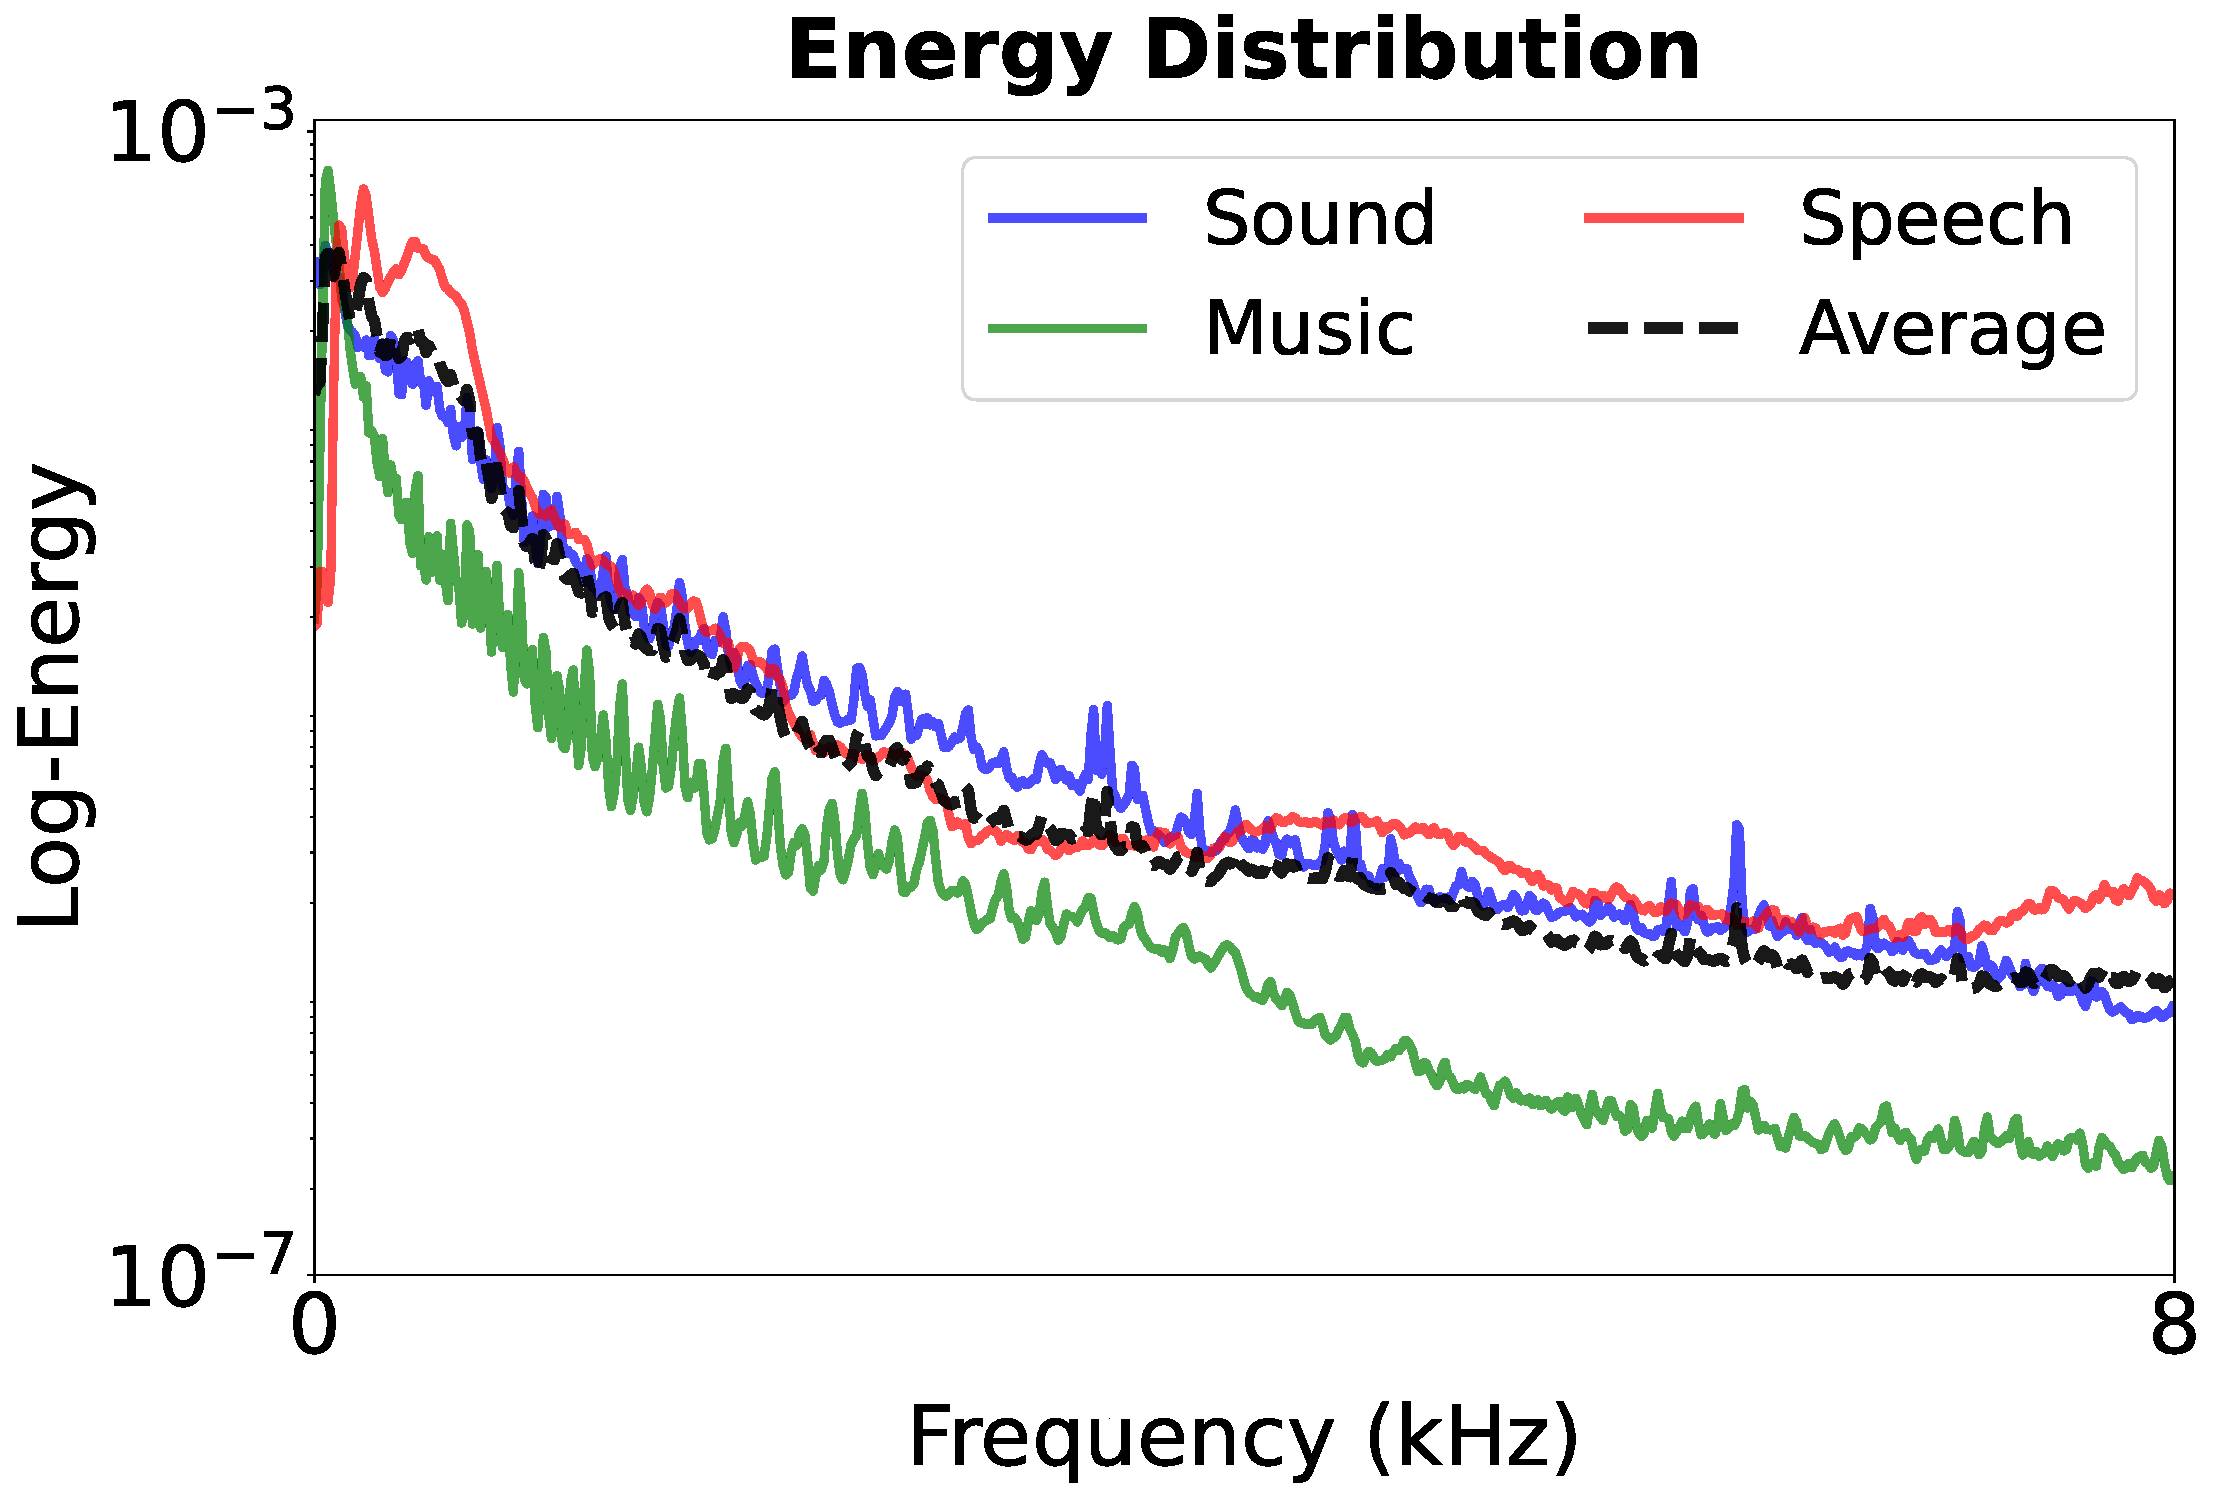
\includegraphics[width=\columnwidth]{pic/energy_spectrum_comparison_log.pdf}
\caption{Frequency domain energy distribution of speech, sound and music (extraction method in Appendix~\ref{app:energy_extraction}). The distributions exhibit significant structural differences across these three domains, demonstrating distinct spectral characteristics.}
\label{fig:energy_spectrum}
\end{figure}


However, the real acoustic world would contain components beyond speech, such as sound and music, all with vastly different acoustic characteristics. As illustrated in Figure~\ref{fig:energy_spectrum}, speech, music, and sound exhibit substantially different average energy distributions across the frequency spectrum. While the aforementioned task-oriented codecs excel on clean speech, their performance degrades significantly~\cite{mousavi2025discrete} when applied to music and sound domains. Given these spectral differences shown in Figure~\ref{fig:energy_spectrum}, it is reasonable that speech codec designs struggle to generalize to music and sound. Current RVQ-based generalized codecs like DAC~\cite{kumar2023high} still exhibit advantages~\cite{mousavi2025discrete} in reconstruction quality for universal audio.

While RVQ-based codecs demonstrate reasonable multi-domain performance, their design could be enhanced. The residual quantization hierarchy lacks explicit acoustic structure, with each layer quantizing residuals that do not correspond to interpretable acoustic attributes. This poses challenges for multi-domain compression: as different audio types have distinct energy distributions (Figure~\ref{fig:energy_spectrum}), a codec handling multiple domains faces a signal source with substantially higher entropy, demanding increased bitrate. Also RVQ applies uniform residual encoding across all domains, requiring the encoder to learn entangled representations for diverse content. Alternative quantization schemes like FSQ~\cite{mentzer2023finite} and GroupVQ~\cite{yang2023hifi} partition along dimensional axes, but these divisions similarly lack grounding in the physical properties of audio signals.

To effectively handle diverse audio domains, we need to account for their structural differences. As shown in Figure~\ref{fig:energy_spectrum}, different domains exhibit substantially different energy distribution across frequency bands. Therefore, band-splitting offers a natural way to decouple these domain-specific structures by processing each frequency band independently. This approach has proven effective in other audio tasks~\cite{luo2023music, yang2021multi}, and a RVQ-based multi-band codec has been successfully built for the speech domain~\cite{ng2025multiband}, which motivate us to adopt similar decomposition principles for universal audio codec design.



% Band-splitting offers a physically meaningful decomposition principle. Classical audio processing has long exploited frequency-domain decomposition, recognizing that different spectral regions carry distinct perceptual and structural information. Recent deep learning approaches, including band-split RNN~\cite{luo2023music} for music source separation and multi-band vocoders for synthesis, have demonstrated that frequency-aligned processing enables more effective modeling by allowing networks to specialize in acoustically coherent spectral regions. Motivated by these insights, we propose to apply band-splitting principles directly to neural codec design, organizing multiple quantization layers according to frequency boundaries rather than residual hierarchies.
% We observe that RVQ's design presents challenges for universal codec development. RVQ employs a cascade of codebooks where each subsequent layer quantizes the residual error of the previous one. While this approach achieves high codebook utilization, the residual information lacks explicit acoustic structure and does not correspond to interpretable attributes like pitch, timbre, or spectral content. This poses particular challenges for multi-domain compression: speech, music, and general audio exhibit fundamentally different spectrotemporal characteristics (e.g., speech has concentrated low-frequency harmonics while music requires full-spectrum fidelity), yet RVQ treats all residuals uniformly across domains. Consequently, the encoder must learn complex, entangled representations to accommodate diverse audio types within the same residual hierarchy, which can lead to less effective reconstruction quality when a single model handles multiple domains.

% This challenge has motivated alternative designs, such as single-layer VQ, which have proven effective for speech. Given the relatively constrained information content of speech signals, a meticulously designed single codebook, paired with a powerful encoder-decoder, can achieve excellent results.(cite wavtokentzer, unicodec) However, this approach does not readily scale to the universal domain. The information content of music and general audio is substantially larger and more diverse, making the efficient utilization of a multi-layer codebook structure a critical, yet unresolved, challenge.
% ORIGINAL:This challenge has motivated alternative designs, such as single-layer VQ, which have proven effective for speech~\cite{ji2024wavtokenizer, jiang2025unicodec}. The quasi-periodic nature and limited spectral bandwidth of speech signals allow a carefully designed single codebook to adequately represent the dominant harmonic structure and formant characteristics. However, extending this to universal audio is nontrivial. Music and general audio exhibit far richer spectrotemporal patterns, including dense harmonic content, broadband transients, and complex polyphonic textures, which exceed the representational capacity of any reasonably-sized single codebook. While multi-layer quantization offers a solution, effectively partitioning and allocating diverse acoustic information across layers in a universal codec remains an open problem.
Motivated by these insights, we propose a band-split codec that decomposes input audio into separate frequency bands, each of which is processed independently and in parallel through dedicated encoder, quantizer, and decoder modules. While band-splitting provides a physically grounded design philosophy, its effective application to codec design requires careful consideration of band configuration and quantization allocation. We conduct extensive experiments to systematically investigate the impact of band count, frequency boundaries, and codebook design on multi-domain codec performance. Through principled design of band partitioning and quantization structure, our approach achieves strong performance across all three domains. Specifically, under the same training conditions, our 2.55 kbps and 3.83 kbps models achieve comparable overall performance to DAC at 4.5 kbps and 6 kbps respectively.

Our contributions can be summarized as follows:
\begin{itemize}
    \item We propose BSCodec, a band-split codec that independently processes time-domain signals from separated frequency bands through parallel encoder-quantizer-decoder modules, achieving strong multi-domain performance through carefully designed band configuration and quantization allocation.
    
    \item Comprehensive experiments on reconstruction quality and downstream tasks demonstrate that BSCodec achieves both perceptual superiority and enhanced effectiveness for audio understanding.

    
\end{itemize}
% ORIGINAL:To address this challenge, we propose an innovative band-split approach for multi-layer codebook organization, which \textbf{demonstrates strong and consistent performance across speech, music, and general audio domains, achieving high reconstruction quality at competitive bitrates with improved parameter efficiency compared to existing universal codecs}. This design leverages the fundamental principle that audio signals naturally decompose into distinct frequency bands, each carrying different perceptual and structural information. Low-frequency bands primarily encode fundamental frequency and harmonic structure, mid-frequency bands capture formants and timbral characteristics, while high-frequency bands contain fine spectral details and transient information. By explicitly partitioning the quantization process along frequency boundaries, our method enables each codebook layer to focus on acoustically coherent information within its designated band, rather than processing opaque residuals. This frequency-aligned decomposition not only facilitates more interpretable representations but also allows the encoder to learn specialized transformations for different spectral regions, leading to more efficient use of codebook capacity and improved reconstruction quality across diverse audio domains.

% Our contributions can be summarized as follows:

% \begin{itemize}
%     \item We propose BSCodec, a unified neural audio codec that achieves strong reconstruction performance across diverse audio types, including speech, music, and general sound. To accomplish this, we introduce a novel multi-layer codebook construction that differs fundamentally from RVQ. Instead of residual quantization, we assign dedicated codebooks to separate frequency bands, enabling more effective allocation of quantization capacity and allowing each encoder to specialize in acoustically coherent spectral regions.
%     \item We demonstrate that our band-split approach generalizes effectively across domains without domain-specific tuning. Through extensive experiments on speech, music, and general audio, we show that a single unified model can match or exceed the performance of domain-specific codecs while maintaining a compact architecture.
%     \item We conduct comprehensive evaluations on both reconstruction quality and downstream task performance, demonstrating that our codec's learned representations are not only perceptually superior but also more effective for various audio understanding tasks, including classification, speaker verification, and emotion recognition.
% \end{itemize}

\section{Related Work}
\label{sec:rel}
\noindent\textbf{Neural Audio Codecs}.
% Neural Audio Codecs (NACs) are designed to compress continuous audio signals into a compact sequence of discrete tokens, aiming for high-quality reconstruction with maximum efficiency in storage and transmission.
% Neural audio codecs (NACs) are designed to compress continuous audio waveforms into compact sequences of discrete tokens while preserving perceptual quality and maximizing storage and transmission efficiency. The dominant paradigm for NACs builds upon the Vector Quantized Variational Autoencoder (VQ-VAE) framework, which comprises three principal components: an encoder that projects input waveforms into a continuous latent space, a vector quantizer that discretizes these representations through nearest-neighbor mapping to learned codebooks, and a decoder that synthesizes audio from the resulting discrete tokens.
The advent of deep learning has enabled significant advances in neural audio compression. They typically adopt the core architecture of RVQ-based discretization paired with GAN~\cite{goodfellow2014generative}-driven reconstruction, and further improve performance via targeted architectural enhancements or optimized training strategies~\cite{zeghidour2021soundstream, defossez2022high, kumar2023high}.

% SoundStream~\cite{zeghidour2021soundstream} proposed a neural codec incorporating Residual Vector Quantization (RVQ) to enhance quantization capacity and Generative Adversarial Networks (GANs)~\cite{goodfellow2014generative} to improve reconstruction quality. Encodec~\cite{defossez2022high} advanced this approach by integrating multi-scale STFT discriminators and a loss-balancing strategy, establishing new benchmarks for perceptual quality. Descript Audio Codec (DAC)~\cite{kumar2023high} further refined RVQ-based architectures through architectural innovations and training strategies, consolidating the residual quantization paradigm as the dominant approach for neural audio compression.

Using a unified model remains challenging due to the distinct energy distribution of universal audio. Recent efforts have pursued universal codecs capable of handling diverse audio types. However, achieving strong multi-domain performance remains challenging due to the distinct acoustic characteristics across domains—speech exhibits narrow-band harmonic structure, music requires wide-band spectral richness, and sound encompasses diverse sound textures~\cite{scharf1970critical}. Existing multi-domain codecs address this heterogeneity through various specialized mechanisms. DAC~\cite{kumar2023high} employs balanced sampling strategies, ensuring each training batch contains data from all three domains (speech, music, sound) to prevent domain bias. 
Further works~\cite{jiang2025unicodec, liu2024semanticodec, yang2025almtokenizer} introduce domain-specific codebooks via Mixture-of-Experts layers~\cite{MoE}, semantic priors and MAE-derived representations~\cite{MAE, huang2022masked}, and more fine-grained supervision to further enhance the language modeling capability of universal audio codecs.
% Unicodec~\cite{jiang2025unicodec} introduces domain-conditioned quantization through Mixture-of-Experts (MoE) layers in the encoder and domain-specific codebook entries, where domain labels explicitly control which codebook vectors are updated during training. SemantiCodec~\cite{liu2024semanticodec} leverages pre-trained AudioMAE~\cite{huang2022masked} representations to inject semantic information for general sound reconstruction. While effective for downstream semantic tasks, these models still lag behind RVQ-based universal codecs in reconstruction quality, and their substantial bitrate differences complicate fair comparison.

In contrast, our work adopts a simpler design philosophy. We employ an architecture and training framework closely aligned with DAC~\cite{kumar2023high}, yet achieve comparable performance for both reconstruction and downstream tasks at half the bitrate on the same dataset. This demonstrates that band-split decomposition offers a simple yet effective alternative for multi-domain codec design, obviating the need for complex domain-specific mechanisms while maintaining strong generalization across audio types.
% The predominant paradigm for NACs is built upon the Vector Quantized-Variational Autoencoder (VQ-VAE) architecture. This framework consists of three main components: an encoder that transforms the input audio waveform into a latent representation, a quantizer that discretizes this representation by mapping it to a finite codebook, and a decoder that reconstructs the audio signal from these discrete tokens.

% To enhance the fidelity and modeling capabilities of this architecture, researchers have widely adopted Residual Vector Quantization (RVQ). This technique utilizes a series of quantization stages, where each subsequent stage quantizes the residual error from the previous one. SoundStream was a pioneering work that successfully integrated RVQ, demonstrating significant improvements in reconstruction quality. Building on this, Encodec further refined the approach by introducing multi-scale discriminators and a sophisticated loss-balancing strategy, setting a new standard for performance. Numerous subsequent works, such as DAC (also known as RVQGAN) and Mimi, have continued to advance and enhance these RVQ-based NACs, solidifying the multi-codebook residual modeling approach as the state-of-the-art for high-quality neural audio compression. In contrast, this work focuses on leveraging frequency bands to enhance the performance of multi-layer codebook codecs.




% The decomposition of an audio signal into distinct frequency bands, or sub-bands, is a widespread technique in audio signal processing. This approach is motivated by the principle that different frequency regions of a signal possess distinct statistical and perceptual characteristics, allowing them to be modeled independently.

% In classical signal processing, this decomposition is commonly achieved through methods such as filter banks—for instance, Quadrature Mirror Filters (QMF)—or time-frequency transformations like the Short-Time Fourier Transform (STFT). These techniques are foundational in domains like audio compression and signal analysis.

% This concept has been integrated into deep learning architectures for various audio tasks. In speech enhancement and source separation, many models operate on a spectrogram representation, implicitly processing different frequency bins separately. Other architectures, like Conv-TasNet, incorporate learnable filter banks as part of the end-to-end network. In the field of audio synthesis and neural coding, band-splitting is employed to allocate modeling resources to different parts of the audio spectrum. For example, some methods utilize separate networks to generate low-frequency and high-frequency content, corresponding to their different acoustic properties.
\begin{figure*}[t]
  \centering
  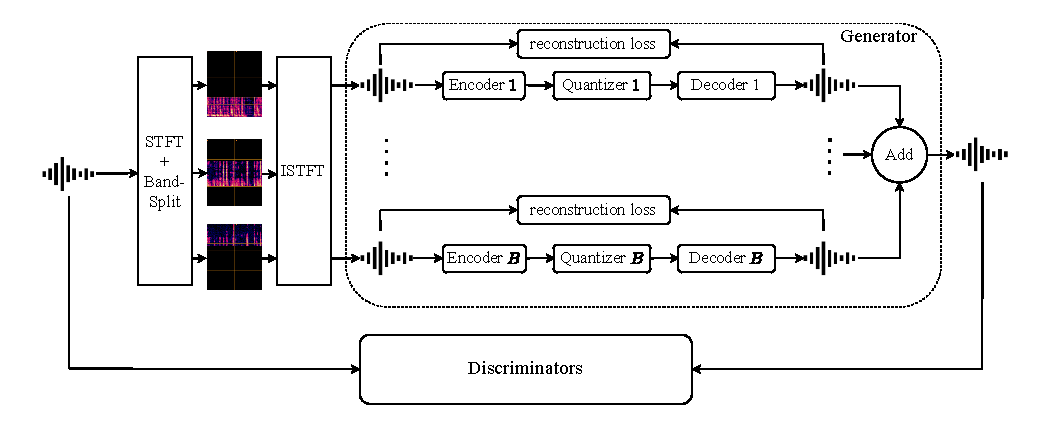
\includegraphics[width=\textwidth]{pic/111.drawio.pdf}
  \caption{BSCodec architecture with band split, multi-band parallel generators and discriminators.}
  \label{fig:wide_architecture}
  \vspace{-10pt}
\end{figure*}


\noindent\textbf{Band-Splitting for Audio Processing}.
% Frequency-domain decomposition of audio signals into distinct sub-bands is a fundamental principle in audio processing, motivated by the observation that different spectral regions exhibit distinct perceptual and structural characteristics that benefit from independent modeling.
% In classical signal processing, band decomposition is realized through filter banks (e.g., QMF) or time-frequency transforms (e.g., STFT, wavelet transforms), forming the foundation for perceptual audio coding standards such as MP3 and AAC. This principle has been increasingly adopted in deep learning. Conv-TasNet introduced learnable filter banks for source separation, demonstrating that adaptive band decomposition can outperform hand-crafted transforms. In neural audio synthesis, multi-band vocoders like HiFi-GAN employ separate branches for low and high frequencies, exploiting their different acoustic properties—low frequencies encode harmonic structure while high frequencies convey texture and transients.
% Recent work has applied band-splitting to neural audio coding. Split-band autoencoders allocate different bitrates to frequency bands based on perceptual importance. However, these approaches primarily focus on signal-level processing or generation. In contrast, our work applies frequency decomposition directly to the quantization structure, organizing multiple codebook layers according to acoustically meaningful spectral partitions rather than residual hierarchies.
Band-splitting decomposes audio signals into separate frequency bands for independent processing, leveraging the observation that different spectral regions carry distinct perceptual and structural information: low frequencies encode harmonic structure and fundamental pitch, mid frequencies capture formants and timbral characteristics, while high frequencies convey transients and texture. This principle has deep roots in classical signal processing. Subband decomposition techniques such as QMF~\cite{malvar1990modulated} and polyphase filter banks~\cite{saramaki2002multirate}, combined with time-frequency transforms like 
MDCT~\cite{prokop2003general}, form the foundation for perceptual audio coding 
standards like MP3~\cite{brandenburg1999mp3} and AAC. Wavelet transforms~\cite{zhang2019wavelet} similarly provide multi-resolution frequency decomposition.


Recent deep learning approaches have demonstrated the effectiveness of band-split architectures across various audio tasks. In music source separation, Band-split RNN~\cite{luo2023music} partitions the spectrogram into multiple frequency bands, processing each band with dedicated recurrent networks before reconstruction. This frequency-aligned decomposition enables the model to specialize in acoustically coherent spectral regions, achieving superior separation quality compared to full-band processing. In neural audio synthesis, Multi-band MelGAN~\cite{yang2021multi} employs separate generator branches for different frequency bands, significantly improving synthesis quality and efficiency by exploiting the distinct acoustic properties of each spectral region.

These successes demonstrate that architectures aligned with the natural spectral structure of audio yield improved performance, providing insights for the design of BSCodec. 

\section{Methodology}
\label{sec:met}
The proposed BSCodec follows an encoder-quantizer-decoder architecture with adversarial training, adopting a framework similar to DAC~\cite{kumar2023high}. The overall architecture is illustrated in Figure \ref{fig:wide_architecture}.

\subsection{Band Splitting}


The model first decomposes the input audio waveform into several band-limited signals through time-frequency domain processing. The input discrete-time signal $x[n]$ is transformed into a spectrogram $X(m, k)$ using the Short-Time Fourier Transform~(STFT):
\begin{equation}
X(m, k) = \sum_{n=0}^{N-1} x[n+mR] w[n] e^{-j2\pi kn/N}
\end{equation}
where $N$ denotes the window length (FFT size), $n$ is the sample index within the window, $w[n]$ denotes the window function, $R$ the hop size, $m$ the frame index, and $k$ the frequency bin index.

The band-splitting operation is then performed directly on $X(m, k)$. For an input sampling rate $f_s = 24$~kHz, we define $B$ non-overlapping frequency bands with boundaries $\{f_0, f_1, \dots, f_B\}$. Each band $b$ is isolated using a binary mask $M_b(k)$:
\begin{equation}
M_b(k) = \begin{cases} 1 & \text{if } f_{b-1} \le \frac{k \cdot f_s}{N} < f_b \\ 0 & \text{otherwise} \end{cases}
\end{equation}
The band-specific spectrogram $X_b(m, k)$ is obtained via element-wise multiplication: $X_b(m, k) = X(m, k) \odot M_b(k)$. Each masked spectrogram is then transformed back to the time domain via Inverse STFT:
% \begin{multline}
% x_b[n] = \sum_{m} w[n-mR] \times \\
% \left( \frac{1}{N} \sum_{k=0}^{N-1} X_b(m, k) e^{j2\pi kn/N} \right)
% \end{multline}
\begin{equation}
\resizebox{\linewidth}{!}{$
x_b[n] = \sum_{m} w[n - mR]\times\left(\frac{1}{N} 
\sum_{k=0}^{N-1} X_b(m, k) e^{j 2\pi k n / N}\right)
$}
\end{equation}


\subsection{Encoder and Decoder}
% In the encoding stage, the input audio is first separated into band-limited waveforms using the STFT/ISTFT process described previously.

% The band-splitting process operates in the frequency domain on the complex spectrogram $X(m, k)$. We first define a set of $B$ non-overlapping frequency intervals, such as $(f_0, f_1), (f_1, f_2), \dots, (f_{B-1}, f_B)$.

% For each band $b$, a binary mask $M_b(k)$ is created and applied across the frequency axis ($k$). The mask's value is 1 for frequency bins falling within the band's range and 0 otherwise. This can be expressed as:

% $$M_b(k) = \begin{cases} 1 & \text{if } f_{b-1} \le \frac{k \cdot \text{sr}}{N} < f_b \\ 0 & \text{otherwise} \end{cases}$$

% Here, $\text{sr}$ is the sampling rate and $N$ is the FFT size. The spectrogram for each band, $X_b(m, k)$, is then isolated by performing an element-wise multiplication of the full spectrogram with the corresponding mask:

% $$X_b(m, k) = X(m, k) \odot M_b(k)$$

% Finally, a separate ISTFT is applied to each of these masked spectrograms, $\{X_1, X_2, \dots, X_B\}$, to yield the set of band-limited waveforms that are fed into the parallel encoders.

The resulting band-limited waveforms $\{x_1[n], x_2[n], \dots, x_B[n]\}$ are processed in parallel by independent encoders. Each encoder adopts the SEANet~\cite{tagliasacchi2020seanet} architecture with downsampling strides of $[2, 4, 5, 8]$ across four stages. Starting from an initial channel dimension of 32 that doubles at each stage, the encoders produce latent features with 512 dimensions at a frame rate of 75~Hz. Each convolutional block contains 3 residual units followed by strided convolution. Critically, no parameters are shared across the $B$ encoders, allowing each to specialize in the spectral characteristics of its frequency range.

The decoder architecture mirrors the encoder with symmetric upsampling strides of $[8, 5, 4, 2]$, progressively upsampling the quantized representations from 512 dimensions back to 24~kHz waveforms. The final output $\hat{x}[n]$ is obtained by summing all band-specific reconstructions: $\hat{x}[n] = \sum_{b=1}^{B} \hat{x}_b[n]$.


\subsection{Vecter Quantization}
The vector quantization stage discretizes the continuous latent representations from each band's encoder into discrete tokens. We employ a single-layer quantization scheme per band, utilizing SimVQ\cite{zhu2024addressing} to accommodate configurations requiring large codebook capacities.

SimVQ\cite{zhu2024addressing} enhances the standard Vector Quantization (VQ) framework by introducing a learnable linear transformation on the codebook embeddings. Given the encoder output $z$ and a codebook of size $K$: $\{\mathbf{c}_1, \mathbf{c}_2, \ldots, \mathbf{c}_K\}$, the quantization proceeds as follows. First, the nearest codebook entry is determined by:
\begin{equation}
q = \arg\min_{\mathbf{c} \in \{\mathbf{c}_1, \ldots, \mathbf{c}_K\}} \|z - \mathbf{c}W\|
\end{equation}
where $W$ is a learnable transformation matrix applied to the codebook embeddings. The quantized representation is then computed as:
\begin{equation}
z_q = z + \text{sg}[qW - z]
\end{equation}
where $\text{sg}[\cdot]$ denotes the stop-gradient operation. During forward propagation, this formulation passes the transformed codebook entry $qW$ to the decoder, while during backpropagation, gradients flow directly through $z$ via the straight-through estimator.

The codebook is optimized through a bidirectional commitment loss with a hyperparameter $\lambda$:
\begin{equation}
\mathcal{L}_{\text{commit}} = \|\text{sg}[z] - qW\|^2 + \lambda \|z - \text{sg}[qW]\|^2
\label{eq:commitment}
\end{equation}
The first term encourages the quantized codes to stay close to the encoder outputs, while the second term allows the encoder to adapt towards the codebook. The transformation matrix $W$ improves optimization dynamics by providing a reparameterization that facilitates gradient-based learning of large codebooks. In our experiments, each band is assigned a SimVQ codebook of size $K = 131{,}072$.


\subsection{Loss Design}

\noindent\textbf{Reconstruction Loss.} We adopt a multi-scale mel-spectrogram L1 loss for frequency-domain reconstruction. Specifically, we compute mel-spectrograms at multiple scales ranging from $2^6$ to $2^{11}$ using a Hann window with 80 mel-frequency bins. To provide better supervision signals for each band, we additionally compute the mel loss between each individual band's reconstructed audio and its corresponding ground-truth band, then average these losses and incorporate them into the overall optimization objective.

\noindent\textbf{Adversarial Loss.} Following DAC~\cite{kumar2023high}, we employ a multi-period discriminator for waveform-level discrimination and a multi-band multi-scale STFT discriminator for frequency-domain discrimination, using the hinge loss formulation with feature matching loss.

\noindent\textbf{Codebook Learning.} The codebook commitment loss follows Equation~\eqref{eq:commitment} with $\lambda$ set to 0.25. Gradients are backpropagated through the codebook lookup using the straight-through estimator.

% \noindent\textbf{Loss weighting}
\noindent\textbf{Loss Weighting.} We set the loss weighting coefficients as follows: 45.0 for the multi-scale mel loss, 2.0 for the feature matching loss, 1.0 for both the adversarial loss and reconstruction loss, and 1.0 for the codebook commitment loss.




% \subsection{Training objective}
% \textbf{Reconstruction Loss} Our reconstruction loss is composed of two key components. The primary component is the multi-scale mel-spectrogram loss from DAC, which measures the L1 distance in the spectral domain at multiple scales. This loss is effective as the mel scale directly relates to perceptual quality, making it preferable to the multi-scale STFT loss. Alongside this spectral objective, we also incorporate a time-domain L1 reconstruction loss.

% \textbf{Reconstruction Loss}
% \textbf{GAN loss} We use the loss function of least-square GAN to train the model, which uses least square loss instead of conventional
% binary cross entropy loss to stabilize training. Additionally, the L1
% feature matching loss proposed in HiFi-GAN is incorporated.


\section{Experiments}
\label{sec:exp}
\subsection{Experimental Stages}
We conduct our experiments in two progressive stages to systematically validate the effectiveness of band split across different domains.

\noindent\textbf{Stage 1: Music Domain Validation.} We first validate the feasibility of band split on music domain. Music is chosen as the initial testbed because its wider fundamental frequency distribution makes it a less challenging learning task for the model. At this stage, we explore various configurations of band split. The experimental results demonstrate that band split achieves excellent performance on music, establishing a strong foundation for further investigation.

\noindent\textbf{Stage 2: Multi-Domain Extension.} Building on the success in music, we extend our investigation to a multi-domain setting encompassing speech, music and sound. We aim to determine whether band split maintains its effectiveness when dealing with diverse acoustic characteristics across domains. Our experiments show that band split remains effective in the multi-domain scenario. Furthermore, we introduce targeted optimizations to enhance model performance across all domains.


\subsection{Datasets}
In Stage 1, we train on Jamendo\cite{bogdanov2019mtg}, MUSDB18\cite{musdb18}, and MAESTRO\cite{hawthorne2018enabling}. We evaluate on two test sets: the MUSDB18 test set for vocal music, and 100 clips from MAESTRO for non-vocal music.

In Stage 2, we train on approximately 2,100 hours of data spanning three domains. For speech, we use LibriTTS~\cite{zen2019libritts}, VCTK~\cite{yamagishi2019vctk}, and CommonVoice~\cite{ardila2019common} as training data, evaluating on the LibriTTS test-clean. For music, we train on Jamendo\cite{bogdanov2019mtg} and MUSDB18\cite{musdb18}, evaluating on the MUSDB18 test set. For sound, we train on AudioSet\cite{gemmeke2017audio} and evaluate on the AudioSet test set. To ensure domain balance, We sample about 700 hours from each domain for training. The detailed dataset distribution after sampling is shown in the Appendix~\ref{app:4}.

% \begin{table*}[t]
% \centering
% \caption{Performance comparison on music and instrument domains}
% \label{tab:music_instrument_results}
% \begin{tabular}{lccccccc}
% \toprule
% \multicolumn{2}{c}{Model} & \multicolumn{3}{c}{Music} & \multicolumn{3}{c}{Instrument} \\
% \cmidrule(lr){1-2} \cmidrule(lr){3-5} \cmidrule(lr){6-8}
% Model & Bitrate & VISQOL$\uparrow$ & Mel Dist.$\downarrow$ & STFT Dist.$\downarrow$ & VISQOL$\uparrow$ & Mel Dist.$\downarrow$ & STFT Dist.$\downarrow$ \\
% \midrule
% DAC & 6 kbps & 4.097 & 0.481 & 1.018 & 4.479 & 0.506 & 0.959 \\
% 5-band VQ & 3.75 kbps & \textbf{4.384} & \textbf{0.445} & \textbf{0.921} & 4.470 & 0.419 & 0.788 \\
% 5-band SimVQ & 3.75 kbps & 4.274 & 0.493 & 1.070 & 4.484 & 0.442 & 0.841 \\
% 3-band SimVQ & 3.825 kbps & 4.196 & 0.477 & 1.042 & 4.495 & \textbf{0.412} & \textbf{0.787} \\
% 2-band SimVQ & 2.55 kbps & 4.104 & 0.482 & 0.994 & 4.484 & 0.417 & 0.806 \\
% RSimVQ & 4.5 kbps & 4.106 & 0.475 & 1.039 & \textbf{4.514} & 0.444 & 0.848 \\
% \bottomrule
% \end{tabular}
% \end{table*}


\begin{table*}[h]
\centering
\small
\setlength{\tabcolsep}{4pt}
\caption{Reconstruction performance of BSCodec and baseline DAC on vocal songs and instrumental music.}
\vspace{-10pt}
\label{tab:music_instrument_results}
\begin{tabular}{lllcccccc}
\toprule
\multicolumn{3}{c}{Model} & \multicolumn{3}{c}{Vocal songs} & \multicolumn{3}{c}{Instrumental music} \\
\cmidrule(lr){1-3} \cmidrule(lr){4-6} \cmidrule(lr){7-9}
Codec & VQ Type & Bitrate & VISQOL$\uparrow$ & Mel Dist.$\downarrow$ & STFT Dist.$\downarrow$ & VISQOL$\uparrow$ & Mel Dist.$\downarrow$ & STFT Dist.$\downarrow$ \\
\midrule
DAC & RVQ & 6.00 kbps & 4.097 & 0.481 & 1.018 & 4.479 & 0.506 & 0.959 \\
DAC & RVQ & 4.50 kbps & 4.075 & 0.493 & 1.025 & 4.459 & 0.517 & 0.962
\\
DAC & RVQ & 3.00 kbps & 4.030 & 0.515 & 1.039 & 4.423 & 0.541 & 0.968
\\
BSCodec & 5-band VQ & 3.75 kbps & \textbf{4.384} & \textbf{0.445} & \textbf{0.921} & 4.470 & 0.419 & 0.788 \\
% BSCodec & 5-band SimVQ & 3.75 kbps & 4.274 & 0.493 & 1.070 & 4.484 & 0.442 & 0.841 \\
BSCodec & 3-band SimVQ & 3.83 kbps & 4.196 & 0.477 & 1.042 & \textbf{4.495} & \textbf{0.412} & \textbf{0.787} \\
BSCodec & 2-band SimVQ & 2.55 kbps & 4.104 & 0.482 & 0.994 & 4.484 & 0.417 & 0.806 \\
% RVQ-Codec(?) & RSimVQ & 4.50 kbps & 4.106 & 0.475 & 1.039 & \textbf{4.514} & 0.444 & 0.848 \\
\bottomrule
\end{tabular}
\vspace{-10pt}
\end{table*}

% \subsection{Training details}
% Our model was built and trained based on the ESPnet framework. The training was conducted with a global batch size of 72, where all audio data was processed into 1-second chunks (corresponding to 24,000 samples). For optimization, we utilized the AdamW optimizer with an initial learning rate of $2.0 \times 10^{-4}$ and betas $(\beta_1, \beta_2)$ set to $(0.5, 0.9)$. This was coupled with an exponential learning rate scheduler, which applied a decay factor of $\gamma = 0.999875$ during training. The total number of training iterations is $340k$.

% \subsection{Band Split}
% We experimented with splitting the signal into 5, 3, and 2 frequency bands. The 5-band configuration splits the signal into $[0, 0.5]$, $[0.5, 2]$, $[2, 4]$, $[4, 8]$, and $[8, 12]$ kHz. For coarser divisions, we tested a 3-band split ($[0, 2]$, $[2, 4]$, $[4, 12]$ kHz) and a 2-band split ($[0, 2]$, $[2, 12]$ kHz). Since configurations with fewer bands require a larger codebook size for each sub-band to maintain quality, we selected SimVQ as our quantization method.

\subsection{Training Setup}
\label{sec:training_details}
Our model is implemented using the codec part~\cite{shi2024espnet} in ESPnet~\cite{watanabe2018espnet} toolkit. We train with a global batch size of 72, processing audio into 1-second chunks at a sampling rate of 24 kHz. We employ the AdamW~\cite{loshchilov2017decoupled} optimizer with an initial learning rate of $2.0 \times 10^{-4}$ and momentum coefficients $(\beta_1, \beta_2) = (0.5, 0.9)$. The learning rate is decayed exponentially with a factor of $\gamma = 0.999875$ per epoch, where each epoch processes 2000 samples (approximately 1200 iterations). Training proceeds for 340k iterations in total.
For comparison, we train a DAC baseline with 8 codebook layers using identical training configurations and datasets. We use the resulting 6 kbps model, along with its 4.5 kbps and 3 kbps variants obtained via codebook dropout, as baselines for comparison.


\subsection{Band Partitioning Configurations}
We investigate band partitioning strategies with 5, 3, and 2 frequency bands. The 5-band configuration partitions the spectrum into $[0, 0.5]$, $[0.5, 2]$, $[2, 4]$, $[4, 8]$, and $[8, 12]$ kHz. For coarser granularities, we evaluate a 3-band configuration ($[0, 2]$, $[2, 4]$, $[4, 12]$ kHz) and a 2-band configuration ($[0, 2]$, $[2, 12]$ kHz). Our partitioning strategy is inspired by the frequency division in band-split RNN~\cite{luo2023music}. While Band-Split RNN uses 41 bands, we adopt only the density distribution of its partitioning. As configurations with fewer bands necessitate larger codebook sizes per sub-band to maintain overall model capacity, we adopt SimVQ\cite{zhu2024addressing} for quantization, which efficiently handles large codebooks.

% \subsection{Metrics}

% \noindent\textbf{Mel-Cepstral Distortion (MCD): }
% The spectral difference between two speech signals by calculating the Euclidean distance between their respective Mel-cepstral coefficients.

% \noindent\textbf{Wide-Band Perceptual Evaluation of Speech Quality (WB-PESQ): }
% It is specified in the ITU-T P.862.2 standard. It predicts the subjective listening quality of a speech signal by comparing the processed version to its original clean reference as an objective metric.

% \noindent\textbf{Short-Time Objective Intelligibility (STOI): }
% The correlation between the short-time temporal envelopes of a processed signal and its clean reference. It's an objective metric.

% \noindent\textbf{Speaker Similarity (SPK\_SIM): }
% We use ESPnet-SPK to compute the cosine similarity between speaker embeddings extracted from the synthesized and ground-truth utterances.

% \noindent\textbf{UTMOS: }
% The University of Tokyo Mean Opinion Score (UTMOS) is a deep learning-based objective metric designed to predict the subjective Mean Opinion Score of a synthesized speech utterance without human listeners.

% \noindent\textbf{VISQOL: }
% Full-reference objective metric that predicts perceived audio quality by measuring the spectro-temporal similarity between a processed signal and its original clean reference.

% \noindent\textbf{Mel Distance: }
% L1 distance between the mel-scaled magnitude spectrograms of the ground truth and the generated sample, where the spectrograms are computed using a multi-resolution STFT with Hann window lengths ranging from $2^6$ to $2^{11}$ and are projected onto an 80-bin Mel filterbank.

% \noindent\textbf{STFT Distance: }
% L1 distance between the ground truth and the prediction, computed using a multiscale STFT with two configurations: a 2048-sample window with a 512-sample hop, and a 512-sample window with a 128-sample hop.

% The Mel Distance and STFT Distance are calculated by adapting our training loss functions. All the other metrics are evaluated with VERSA.

% \subsection{Evaluation Metrics}

% We employ the following metrics for comprehensive evaluation across different audio domains.

% \noindent\textbf{Speech Quality Metrics:}
% \begin{itemize}
%     \item \textbf{Mel-Cepstral Distortion (MCD)}. Measures spectral difference by calculating the Euclidean distance between Mel-cepstral coefficients of two speech signals.
    
%     \item \textbf{Wide-Band PESQ (WB-PESQ)}. An ITU-T P.862.2 standard metric that predicts subjective listening quality by comparing processed speech to its clean reference.
    
%     \item \textbf{Short-Time Objective Intelligibility (STOI)}. Evaluates speech intelligibility by measuring correlation between short-time temporal envelopes of processed and reference signals.
    
%     \item \textbf{Speaker Similarity (SPK\_SIM)}. Computed using ESPnet-SPK as the cosine similarity between speaker embeddings extracted from synthesized and ground-truth utterances.
    
%     \item \textbf{UTMOS}. A deep learning-based metric from the University of Tokyo that predicts Mean Opinion Score without human listeners.
% \end{itemize}

% \noindent\textbf{Audio and Music Quality Metrics:}
% \begin{itemize}
%     \item \textbf{VISQOL}. A full-reference metric predicting perceived audio quality through spectro-temporal similarity analysis.
    
%     \item \textbf{Mel Distance}. L1 distance between mel-scaled magnitude spectrograms computed using multi-resolution STFT (window lengths from $2^6$ to $2^{11}$ samples with Hann windows, projected onto an 80-bin Mel filterbank).
    
%     \item \textbf{STFT Distance}. L1 distance computed using multi-scale STFT with two configurations: (1) 2048-sample window with 512-sample hop, and (2) 512-sample window with 128-sample hop.
% \end{itemize}

% \noindent Mel Distance and STFT Distance are adapted from our training loss functions. All other metrics are evaluated using the VERSA toolkit.

\subsection{Evaluation Metrics}

We evaluate our model using domain-specific metrics. For speech, we use Mel Cepstral Distortion (MCD), WB-PESQ~\cite{rix2001perceptual}, STOI~\cite{taal2010short}, Speaker Similarity (SPK\_SIM)\cite{jung2024espnet} and UTMOS~\cite{saeki2022utmos}. For audio and music, we use VISQOL\cite{hines2015visqol}, Mel Distance and STFT Distance. All metrics except Mel Distance and STFT Distance are evaluated using the VERSA~\cite{shi2024versa} toolkit with default configurations.

\noindent\textbf{Mel Distance} is computed as the L1 distance between mel-scaled magnitude spectrograms using multi-resolution STFT with Hann window lengths ranging from $2^6$ to $2^{11}$ samples projected onto an 80-bin Mel filterbank.

\noindent\textbf{STFT Distance} is computed as the L1 distance using multi-scale STFT with a 2048-sample window and 512-sample hop as well as a 512-sample window and 128-sample hop.

% \begin{table*}[t]
% \centering
% \scriptsize
% \setlength{\tabcolsep}{2pt}
% \caption{Performance comparison on speech, audio and music domains}
% \label{tab:reconstruction_results}
% \begin{tabular}{lllccccccccccc}
% \toprule
% \multicolumn{3}{c}{Model} & \multicolumn{5}{c}{Speech} & \multicolumn{3}{c}{Audio} & \multicolumn{3}{c}{Music} \\
% \cmidrule(lr){1-3} \cmidrule(lr){4-8} \cmidrule(lr){9-11} \cmidrule(lr){12-14}
% Codec & VQ Type & Bitrate & MCD$\downarrow$ & PESQ$\uparrow$ & STOI$\uparrow$ & SPK\_SIM$\uparrow$ & UTMOS$\uparrow$ & VISQOL$\uparrow$ & Mel Dist.$\downarrow$ & STFT Dist.$\downarrow$ & VISQOL$\uparrow$ & Mel Dist.$\downarrow$ & STFT Dist.$\downarrow$ \\
% \midrule
% DAC & RVQ & 6.00 kbps & 5.40 & \textbf{2.915} & \textbf{0.934} & 0.751 & 3.356 & 4.085 & \textbf{0.452} & 0.874 & 4.201 & \textbf{0.439} & 0.974 \\
% DAC & RVQ & 4.50 kbps & 5.50 & 2.726 & 0.925 & 0.734 & 3.201 & 4.055 & 0.463 & 0.880 & 4.171 & 0.449 & 0.979 \\
% BSCodec & 5\# VQ & 3.75 kbps & 5.08 & 1.961 & 0.894 & 0.810 & 2.515 & \textbf{4.245} & 0.463 & 0.800 & \textbf{4.326} & 0.464 & 0.892 \\
% BSCodec & 3\# SimVQ & 3.83 kbps & \textbf{5.05} & 2.544 & 0.920 & \textbf{0.852} & \textbf{3.360} & 4.234 & 0.456 & \textbf{0.794} & 4.298 & 0.461 & \textbf{0.888} \\
% BSCodec & 2\# SimVQ & 2.55 kbps & 5.42 & 2.429 & 0.916 & 0.783 & 3.304 & 4.137 & 0.470 & 0.846 & 4.166 & 0.479 & 0.916 \\
% \bottomrule
% \end{tabular}
% \end{table*}



% \begin{table*}[t]
% \centering
% \caption{Performance comparison on speech domain}
% \label{tab:speech_results}
% \begin{tabular}{lcccccc}
% \toprule
% \multicolumn{2}{c}{Model} & \multicolumn{5}{c}{Speech} \\
% \cmidrule(lr){1-2} \cmidrule(lr){3-7}
% Model & Bitrate & MCD$\downarrow$ & PESQ$\uparrow$ & STOI$\uparrow$ & SPK\_SIM$\uparrow$ & UTMOS$\uparrow$ \\
% \midrule
% DAC & 6.00 kbps & 5.40 & \textbf{2.915} & \textbf{0.934} & 0.751 & 3.356 \\
% DAC & 4.50 kbps & - & - & - & - & - \\
% RSimVQ & 4.50 kbps & 6.00 & 2.462 & 0.906 & 0.662 & 2.655 \\
% 5-band VQ & 3.75 kbps & 5.08 & 1.961 & 0.894 & 0.810 & 2.515 \\
% 5-band SimVQ & 3.75 kbps & 5.66 & 2.030 & 0.892 & 0.774 & 2.723 \\
% 3-band SimVQ & 3.83 kbps & \textbf{5.05} & 2.544 & 0.920 & \textbf{0.852} & \textbf{3.360} \\
% 2-band SimVQ & 2.55 kbps & 5.42 & 2.429 & 0.916 & 0.783 & 3.304 \\
% \bottomrule
% \end{tabular}
% \end{table*}
% \begin{table*}[t]
% \centering
% \setlength{\tabcolsep}{4pt}
% \caption{Performance comparison on speech domain}
% \label{tab:speech_results}
% \begin{tabular}{lllccccc}
% \toprule
% \multicolumn{3}{c}{Model} & \multicolumn{5}{c}{Speech} \\
% \cmidrule(lr){1-3} \cmidrule(lr){4-8}
% Codec & VQ Type & Bitrate & MCD$\downarrow$ & PESQ$\uparrow$ & STOI$\uparrow$ & SPK\_SIM$\uparrow$ & UTMOS$\uparrow$ \\
% \midrule
% DAC & RVQ & 6.00 kbps & 5.40 & \textbf{2.915} & \textbf{0.934} & 0.751 & 3.356 \\
% DAC & RVQ & 4.50 kbps & 5.50 & 2.726 & 0.925 & 0.734 & 3.201 \\
% % RVQ-Codec(?) & RSimVQ & 4.50 kbps & 6.00 & 2.462 & 0.906 & 0.662 & 2.655 \\
% BSCodec & 5-band VQ & 3.75 kbps & 5.08 & 1.961 & 0.894 & 0.810 & 2.515 \\
% % BSCodec & 5-band SimVQ & 3.75 kbps & 5.66 & 2.030 & 0.892 & 0.774 & 2.723 \\
% BSCodec & 3-band SimVQ & 3.83 kbps & \textbf{5.05} & 2.544 & 0.920 & \textbf{0.852} & \textbf{3.360} \\
% BSCodec & 2-band SimVQ & 2.55 kbps & 5.42 & 2.429 & 0.916 & 0.783 & 3.304 \\
% \bottomrule
% \end{tabular}
% \end{table*}

\section{Results and Discussions}
\label{sec:res}

\subsection{Music Reconstruction}
\label{sec:musrec}
% 我们首先在基频分布较广的music domain上进行实验，（这个domain相比3个domain mix难度要小很多，在appendix里面会补充），我们尝试了多种划分，见表格1。可以看到，划分成5个band的配置取得了最好的表现。（一顿分析）这说明band划分至少在music这种基频分布较广的domain上是很有效的，由于单纯采用residual VQ的DAC。（如果文章总篇幅过长，可能在music的实验结果表格上可以直接先把SimVQ去了，毕竟在故事上是为了在语音上表现也好才提出的SimVQ大码本少band的权衡）
% \red{We first conduct experiments on the music domain, which exhibits a broad fundamental frequency distribution. (This domain is considerably less challenging compared to a mixture of three domains, with supplementary results provided in the appendix.) We explore various partitioning configurations, as shown in Table 1. The results demonstrate that the configuration with 5 bands achieves the best performance. (Analysis of the results indicates...) This suggests that band partitioning is highly effective, at least for domains like music that feature a wide fundamental frequency distribution, compared to DAC which solely employs residual VQ. (Refer to the Chinese annotations for details.)}
% To compare the performance of our model with existing RVQ-based models on the same domain, we trained a DAC model using the same dataset and training configurations as our model. We set the number of codebook layers to 8, corresponding to a bitrate of 6~kbps, and employed quantizer dropout during training. We utilized the trained DAC model with 8 layers and the first 6 layers, corresponding to bitrates of 6~kbps and 4.5~kbps respectively, as baselines. We conducted evaluations on two datasets: one containing music with vocals, and the other consisting of solo piano performances (instrument). We compared the performance across these two datasets using three metrics: VISQOL, Mel Distance, and STFT Distance.

% As can be observed, in terms of reconstruction quality, the 5-band model achieves significantly superior performance compared to the baseline DAC model on this domain, while operating at a lower bitrate of 3.75~kbps.

We first evaluate on the music domain, which exhibits a broad fundamental frequency distribution. We compare against the DAC baselines described in Section~\ref{sec:training_details}. We assess reconstruction quality on vocal music and solo piano datasets using VISQOL, Mel Distance, and STFT Distance metrics.

As shown in Table~\ref{tab:music_instrument_results}, our 5-band VQ configuration achieves the best performance on music at 3.75 kbps compared to both DAC baselines, demonstrating that fine-grained frequency decomposition effectively captures harmonic content. On the instrument domain, the 3-band SimVQ achieves competitive results at 3.83 kbps, while the 2-band configuration maintains strong performance at only 2.55 kbps. These results demonstrate that band partitioning is highly effective for domains with wide frequency distributions, with optimal granularity varying by domain complexity.

\begin{table*}[t]
\centering
\scriptsize
\setlength{\tabcolsep}{2pt}
\caption{Reconstruction performance on speech, sound and music domains. $\dagger$ means the official release.}
\vspace{-10pt}
\label{tab:reconstruction_results}
\begin{tabular}{lllccccccccccc}
\toprule
\multicolumn{3}{c}{Model} & \multicolumn{5}{c}{Speech} & \multicolumn{3}{c}{Sound} & \multicolumn{3}{c}{Music} \\
\cmidrule(lr){1-3} \cmidrule(lr){4-8} \cmidrule(lr){9-11} \cmidrule(lr){12-14}
Codec & VQ Method & Bitrate & MCD$\downarrow$ & PESQ$\uparrow$ & STOI$\uparrow$ & SPK\_SIM$\uparrow$ & UTMOS$\uparrow$ & VISQOL$\uparrow$ & Mel Dist.$\downarrow$ & STFT Dist.$\downarrow$ & VISQOL$\uparrow$ & Mel Dist.$\downarrow$ & STFT Dist.$\downarrow$ \\
\midrule
EnCodec$^\dagger$ & RVQ & 6.00 kbps & 5.94 & 2.715 & 0.939 & 0.865 & 3.038 & 4.240 & 0.485 & 0.940 & 4.410 & 0.435 & 0.980 \\
DAC & RVQ & 6.00 kbps & 5.40 & 2.915 & 0.934 & 0.751 & 3.356 & 4.085 & 0.452 & 0.874 & 4.201 & 0.439 & 0.974 \\
\midrule
DAC & RVQ & 4.50 kbps & 5.50 & \textbf{2.726} & \textbf{0.925} & 0.734 & 3.201 & 4.055 & 0.463 & 0.880 & 4.171 & \textbf{0.449} & 0.979 \\
DAC & RVQ & 3.00 kbps & 5.74 & 2.397 & 0.905 & 0.686 & 2.869 & 3.990 & 0.485 & 0.893 & 4.105 & 0.472 & 0.993 \\
EnCodec$^\dagger$ & RVQ & 3.00 kbps & 6.49 & 2.048 & 0.901 & 0.771 & 2.305 & 4.085 & 0.531 & 0.978 & 4.262 & 0.481 & 1.014 \\
BSCodec & 5\# VQ & 3.75 kbps & 5.08 & 1.961 & 0.894 & 0.810 & 2.515 & \textbf{4.245} & 0.463 & 0.800 & \textbf{4.326} & 0.464 & 0.892 \\
BSCodec & 3\# SimVQ & 3.83 kbps & \textbf{5.05} & 2.544 & 0.920 & \textbf{0.852} & \textbf{3.360} & 4.234 & \textbf{0.456} & \textbf{0.794} & 4.298 & 0.461 & \textbf{0.888} \\
BSCodec & 2\# SimVQ & 2.55 kbps & 5.42 & 2.429 & 0.916 & 0.783 & 3.304 & 4.137 & 0.470 & 0.846 & 4.166 & 0.479 & 0.916 \\
\bottomrule
\end{tabular}
\vspace{-10pt}
\raggedright
\end{table*}
% \begin{table*}[t]
% \centering
% \small
% \setlength{\tabcolsep}{4pt}
% \caption{Performance comparison on audio and music domains}
% \label{tab:audio_music_results}
% \begin{tabular}{lllcccccc}
% \toprule
% \multicolumn{3}{c}{Model} & \multicolumn{3}{c}{Audio} & \multicolumn{3}{c}{Music} \\
% \cmidrule(lr){1-3} \cmidrule(lr){4-6} \cmidrule(lr){7-9}
% Codec & VQ Type & Bitrate & VISQOL$\uparrow$ & Mel Dist.$\downarrow$ & STFT Dist.$\downarrow$ & VISQOL$\uparrow$ & Mel Dist.$\downarrow$ & STFT Dist.$\downarrow$ \\
% \midrule
% DAC & RVQ & 6.00 kbps & 4.085 & \textbf{0.452} & 0.874 & 4.201 & \textbf{0.439} & 0.974 \\
% DAC & RVQ & 4.50 kbps & 4.055 & 0.463 & 0.880 & 4.171 & 0.449 & 0.979 \\
% % RVQ-Codec(?) & RSimVQ & 4.50 kbps & 4.068 & 0.469 & 0.851 & 4.172 & 0.444 & 0.899 \\
% BSCodec & 5-band VQ & 3.75 kbps & \textbf{4.245} & 0.463 & 0.800 & \textbf{4.326} & 0.464 & 0.892 \\
% % BSCodec & 5-band SimVQ & 3.75 kbps & 4.185 & 0.476 & 0.814 & 4.267 & 0.476 & 0.903 \\
% BSCodec & 3-band SimVQ & 3.83 kbps & 4.234 & 0.456 & \textbf{0.794} & 4.298 & 0.461 & \textbf{0.888} \\
% BSCodec & 2-band SimVQ & 2.55 kbps & 4.137 & 0.470 & 0.846 & 4.166 & 0.479 & 0.916 \\
% \bottomrule
% \end{tabular}
% \end{table*}


\subsection{Multi-domain Reconstruction}
\label{sec:mdrec}
% 基频分布极窄的speech domain对band split提出了很大的挑战，我们用相同的5band的配置尝试在speech、music、audio三个domain混合的数据集上进行训练，观察效果。根据表2可以看到，5band split在speech上的表现并不理想。虽然整个音频的MCD很低，也就是频谱包络和原来的相似度很高，但是从更接近人类听感的PESQ，STOI，UTMOS等指标可以看到，语音的基频信息还是没能很好的保留（这句话说的有点主观，可能要换个说法）。（怎么解释一下强行在低频划分更密的band很困难，或者干脆不提这个防止被审稿人问）。为了缓解这个问题，我们的想法是，不对低频进行过分刻意的划分，而是用一个更大的码本去处理这个划分不那么密的低频部分。同时高频保持着原有的划分。而SimVQ是处理大码本很好的量化方法（这个在method里面肯定提了，可能冗余）观察table2，可以看到，这种改良在speech domain上取得了出色的表现，同时，配合高频上很好的重构表现（很好的重构了高频共振峰、摩擦音和爆破音），在Speaker Similarity上取得了极其出色的表现。
% 不仅在speech上有出色的表现，我们也可以看table3，在audio和music上的表现，可以看到，5band依然在audio和music上取得了最好的效果，而换成3band以后几乎没有性能损失！

% \red{The speech domain, characterized by an extremely narrow fundamental frequency distribution, poses significant challenges for band splitting. We employ the same 5-band configuration to train on a dataset mixing speech, music, and audio domains, and evaluate the performance. As shown in Table 1, the 5-band split yields suboptimal results on speech. Although the overall MCD (Mel Cepstral Distortion) is low, indicating high similarity in spectral envelope, perceptually-oriented metrics such as PESQ, STOI, and UTMOS reveal that the fundamental frequency information of speech is not well preserved. To address this issue, rather than forcing overly fine-grained partitioning in the low-frequency range, we adopt a larger codebook to handle the less densely partitioned low-frequency region, while maintaining the original partitioning for high frequencies. SimVQ serves as an effective quantization method for handling large codebooks. As observed in Table 1, this modification achieves superior performance on the speech domain. Moreover, combined with excellent reconstruction of high-frequency components (such as formants, fricatives, and plosives), it demonstrates exceptional performance in speaker similarity.}

% \red{Beyond the remarkable results on speech, Table 3 presents the performance on audio and music domains. The 5-band configuration still achieves the best results on audio and music. Notably, when switching to 3 bands, there is virtually no performance degradation.}
% \red{See Chinese annotations.}
% We conducted experiments on a strictly balanced dataset comprising three domains: speech, audio, and music. We adopted the same model architecture used for music and trained the model accordingly, while also training a DAC model as the baseline. For speech evaluation, we employed MCD, WB-PESQ, STOI, SPK\_SIM, and UTMOS as metrics. For both audio and music domains, we utilized VISQOL, Mel Distance, and STFT Distance for assessment. The results reveal that the 5-band decomposition, which demonstrated excellent performance on music, failed to achieve satisfactory results on speech. Given that the fundamental frequency range of speech is narrower and more concentrated compared to music, our experiments indicate that attempting to split low frequencies into multiple bands with fixed codebook sizes struggles to yield good performance on speech. Consequently, for speech, we preserve the low-frequency region as a unified entity and allocate a large codebook using SimVQ, thereby maintaining the representational capacity of this component. Experimental results demonstrate that this approach achieves excellent performance on speech, while the effectiveness of high-frequency splitting (as validated by experiments on the music domain) ensures that the model continues to exhibit outstanding performance on both audio and music domains.

% We conduct experiments on a strictly balanced dataset comprising three domains: speech, audio, and music. We train our model alongside a DAC baseline using identical configurations. For speech evaluation, we employ MCD, WB-PESQ, STOI, speaker similarity (SPK\_SIM), and UTMOS as metrics. For audio and music domains, we utilize VISQOL, Mel Distance, and STFT Distance.

% As shown in Table~\ref{tab:reconstruction_results}, the speech domain, characterized by a narrow and concentrated fundamental frequency range, poses significant challenges for band splitting. While the 5-band VQ configuration achieves excellent results on audio (VISQOL: 4.245) and music (VISQOL: 4.326), it yields suboptimal performance on speech. Although MCD remains competitive at 5.08, perceptually-oriented metrics reveal limitations: PESQ of 1.961, STOI of 0.894, and UTMOS of 2.515, all substantially lower than the DAC baseline.

% To address this challenge, we adopt a coarser partitioning strategy for speech. Rather than forcing fine-grained low-frequency decomposition, we employ the 3-band SimVQ configuration, which uses a larger codebook to handle a unified low-frequency region while maintaining high-frequency splitting. This modification achieves substantial improvements on speech: PESQ increases to 2.544, STOI to 0.920, and UTMOS to 3.360, with speaker similarity reaching 0.852 compared to DAC's 0.734. The enhanced speaker similarity demonstrates that our approach effectively preserves speaker-specific characteristics, particularly through the improved low-frequency representation combined with accurate high-frequency reconstruction of formants, fricatives, and plosives.

% Notably, the 3-band configuration maintains competitive performance on audio and music domains, with virtually no degradation compared to the 5-band variant. This demonstrates that our adaptive partitioning strategy successfully balances the trade-off between speech-specific requirements and multi-domain effectiveness. The 2-band configuration further reduces bitrate to 2.55 kbps while maintaining reasonable performance across all domains, offering an efficient alternative for bandwidth-constrained scenarios.

We conduct experiments on a strictly balanced dataset comprising three domains: speech, audio, and music. We train our model alongside a DAC baseline using identical configurations. For speech evaluation, we employ MCD, WB-PESQ, STOI, SPK\_SIM and UTMOS as metrics. For audio and music domains, we utilize VISQOL, Mel Distance and STFT Distance.

As shown in Table~\ref{tab:reconstruction_results}, the speech domain, characterized by a narrow and concentrated fundamental frequency range, poses significant challenges for band splitting. While the 5-band VQ configuration achieves excellent results on audio and music domains, it yields suboptimal performance on speech. Although MCD remains competitive, perceptually-oriented metrics reveal substantial limitations compared to the DAC baseline.


To address this challenge, we adopt a coarser partitioning strategy for speech. Rather than forcing fine-grained low-frequency decomposition, we employ the 3-band SimVQ configuration at 3.83 kbps, which uses a larger codebook to handle a unified low-frequency region while maintaining high-frequency splitting. This modification achieves substantial improvements on speech across all perceptual metrics, with speaker similarity significantly outperforming the DAC baseline. The enhanced speaker similarity demonstrates that our approach effectively preserves speaker-specific characteristics, particularly through the improved low-frequency representation combined with accurate high-frequency reconstruction of formants, fricatives, and plosives.

Notably, the 3-band configuration maintains competitive performance on audio and music domains, with virtually no degradation compared to the 5-band variant. This demonstrates that our adaptive partitioning strategy successfully balances the trade-off between speech-specific requirements and multi-domain effectiveness. The 2-band configuration further reduces bitrate to 2.55 kbps while maintaining reasonable performance across all domains, offering an efficient alternative for bandwidth-constrained scenarios.

\begin{table*}[t]
\centering
\small
\setlength{\tabcolsep}{4pt}
\renewcommand{\arraystretch}{0.95}
\caption{Performance comparison on ARCH.}
\vspace{-10pt}
\label{tab:classification_results_2}
\begin{tabular}{llccccccc}
\toprule
\multicolumn{2}{c}{Model} & \multicolumn{2}{c}{Speech} & \multicolumn{3}{c}{Audio} & \multicolumn{2}{c}{Music} \\
\cmidrule(lr){1-2} \cmidrule(lr){3-4} \cmidrule(lr){5-7} \cmidrule(lr){8-9}
Model & \# Enc. & RAVDESS$\uparrow$ & AM$\uparrow$ & ESC-50$\uparrow$ & US8K$\uparrow$ & VIVAE$\uparrow$ & MTT$\uparrow$ & MS-DB$\uparrow$ 
\\
\midrule
DAC & 1 & 0.3958 & 0.7791 & 0.3335 & 0.5311 & 0.3285 & 0.2949 & 0.5754 \\
BSCodec & 2 & 0.4201 & 0.7801 & 0.3795 & 0.5798 & 0.3265 & \textbf{0.3555} & \textbf{0.7021} 
\\
BSCodec & 3 & 0.4306 & 0.7759 & 0.3725 & 0.5654 & 0.3258 & 0.3531 & 0.6969 
\\
BSCodec & 5 & \textbf{0.5069} & \textbf{0.8548} & \textbf{0.3930} & \textbf{0.5956} & \textbf{0.3810} & 0.2580 & 0.5751
\\
\bottomrule
\end{tabular}
\vspace{-10pt}
\end{table*}

% As shown in Figure~\ref{fig:codebook_analysis}, despite achieving significantly better reconstruction quality than DAC, our model maintains comparable overall codebook utilization (98.63\% for DAC vs. 92.84\% for BSCodec-3band). We further analyze the joint utilization of adjacent codebook layers following the methodology described in the method section. The results reveal that the joint utilization of DAC's first two layers is comparable to our large single codebook. For DAC, as residual layers progress, the encoded information approaches random noise, resulting in increasingly high utilization rates.

\subsection{Codebook Utilization}

We evaluate codebook utilization on models trained across three domains. We collect statistics on codebook usage frequencies using a test set comprising LibriTTS test-clean and test-other, AudioSet test set, and MUSDB18 test set, totaling 237k seconds of audio data. As shown in Figure~\ref{fig:codebook_analysis}, when examining per-layer utilization, our model exhibits slightly lower rates than DAC (98.63\% for DAC vs. 92.84\% for BSCodec-3band). To analyze inter-codebook correlations, we compute joint utilization by combining codewords from two adjacent codebooks into a larger codebook. The calculation methods for single-layer and joint codebook utilization are detailed in Appendix~\ref{app:2}. The joint utilization for each pair of adjacent codebooks is shown in Figure~\ref{fig:codebook_analysis}. The layer-wise growth pattern remains consistent with single-layer observations, but notably, DAC's first two layers exhibit strong correlation, achieving the same joint utilization to our single-layer SimVQ. Moreover, DAC's final two layers show very high joint utilization. However, reconstruction results demonstrate that DAC's final two layers, despite exhibiting very high joint utilization (totaling 20 bits), contribute minimally to performance improvement. In contrast, when we reduce our model from 3-band to 2-band by removing the 17-bit codebook in the high-frequency region, speech performance degrades only slightly at 2.55 kbps, but notable performance gaps emerge in both audio and music domains compared to the 3-band configuration. This suggests that our band-specific codebooks capture domain-critical information more effectively than residual quantization approaches.

\begin{figure}[t]
\centering
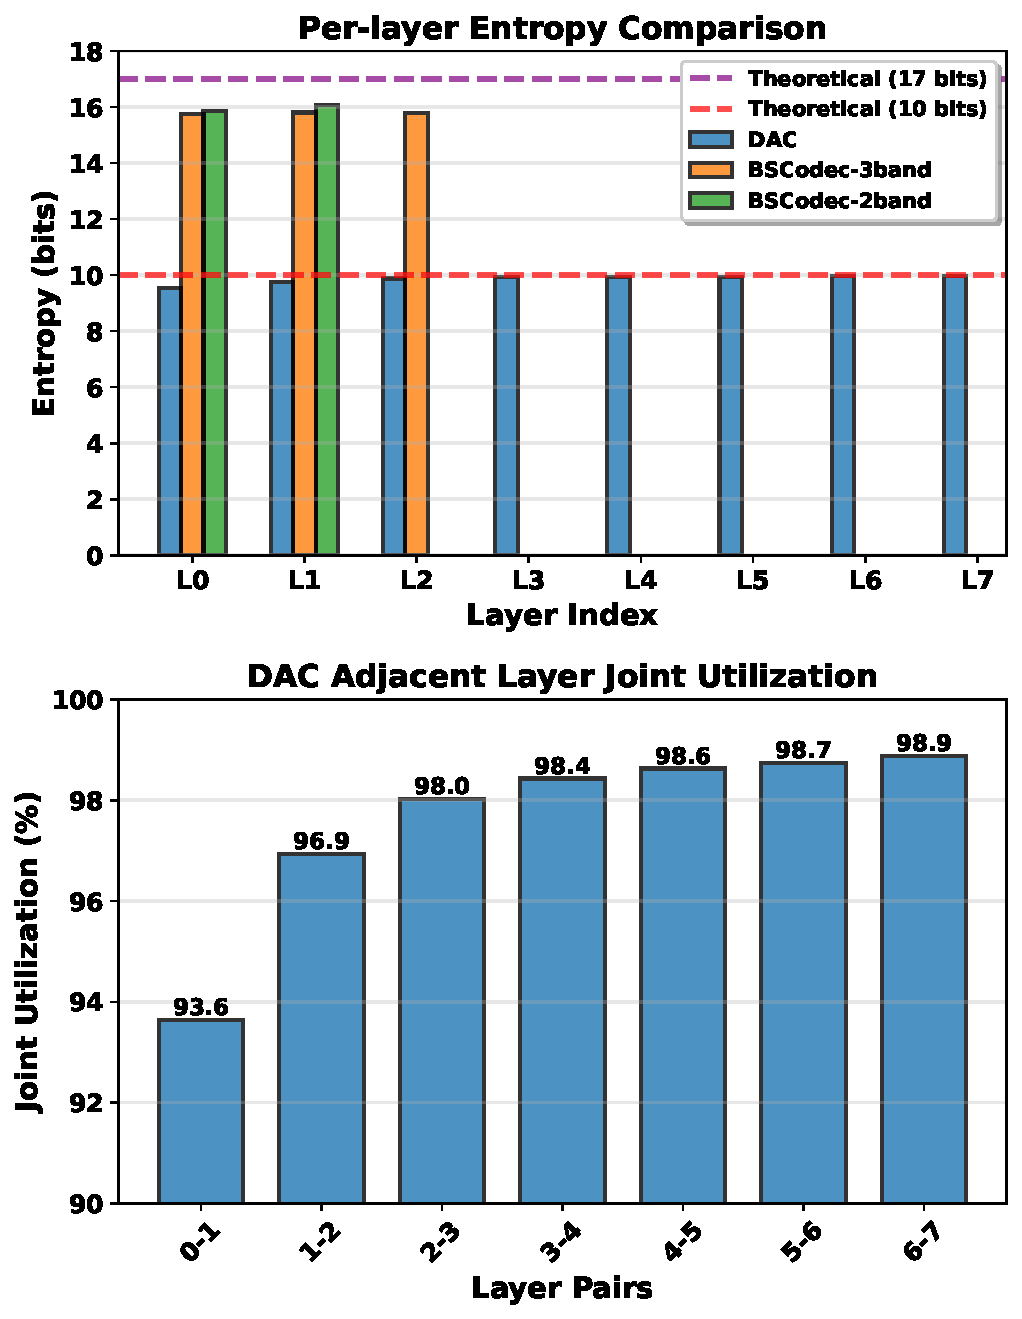
\includegraphics[width=\columnwidth]{pic/codebook_analysis_vertical2.pdf}
\caption{Codebook utilization analysis. Top: Per-layer entropy comparison across different models. Bottom: Joint utilization of adjacent layers in DAC.}
\label{fig:codebook_analysis}
\vspace{-10pt}
\end{figure}


% However, reconstruction results demonstrate that DAC's final two layers, despite exhibiting very high joint utilization (totaling 20 bits), contribute minimally to performance improvement. In contrast, when we reduce our model from 3-band to 2-band by removing the 17-bit codebook in the high-frequency region, speech performance degrades only slightly at 2.55 kbps, but notable performance gaps emerge in both audio and music domains compared to the 3-band configuration. This suggests that our band-specific codebooks capture domain-critical information more effectively than residual quantization approaches.

% \begin{table*}[htbp]
% \centering
% \caption{Performance on downstream tasks}
% \label{tab:downstream_results}
% \begin{tabular}{lllcccc}
% \toprule
% & & & \multicolumn{3}{c}{Speech} & Audio \\
% \cmidrule(lr){4-6} \cmidrule(lr){7-7}
% Model & VQ Type & Bitrate & ACC(ER)$\uparrow$ & EER(ASV)$\downarrow$ & WER(ASR)$\downarrow$ & mAP(AEC)$\uparrow$ \\
% \midrule
% DAC & RVQ & 6.00 kbps & 72.36\% & 3.94\% & \textbf{4.1\%} & 78.15\% \\
% DAC & RVQ & 4.50 kbps & 71.74\% & 4.46\% & 4.3\% & 74.90\% \\
% % RSimVQ & 70.49\% & 6.23\% & 5.32\% & 75.40\% \\
% BSCodec & 5-band VQ & 3.75 kbps & 67.01\% & 4.01\% & 4.73\% & 82.85\% \\
% BSCodec & 2-band SimVQ & 2.55 kbps & 71.11\% & 4.18\% & 4.62\% & 85.00\% \\
% BSCodec & 3-band SimVQ & 3.83 kbps & \textbf{73.26\%} & \textbf{2.67\%} & 4.4\% & \textbf{87.95\%} \\
% \bottomrule
% \end{tabular}
% \end{table*}



\subsection{Downstream task}
\label{sec:down}
%考虑把table4变成单栏表格
% \red{Consider turning table4 into a single-column table}
% \begin{table*}[htbp]
% \centering
% \caption{Performance on downstream tasks}
% \label{tab:downstream_results}
% \begin{tabular}{lcccc}
% \toprule
% & \multicolumn{3}{c}{Speech} & Audio \\
% \cmidrule(lr){2-4} \cmidrule(lr){5-5}
% Model & ACC(ER)$\uparrow$ & EER(ASV)$\downarrow$ & WER(ASR)$\downarrow$ & mAP(AEC)$\uparrow$ \\
% \midrule
% DAC 6 kbps & 72.36\% & 3.94\% & \textbf{4.1\%} & 78.15\% \\
% DAC 4.5 kbps & 71.74\% & 4.46\% & 4.3\% & 74.90\% \\
% % RSimVQ & 70.49\% & 6.23\% & 5.32\% & 75.40\% \\
% 3-band SimVQ & \textbf{73.26\%} & \textbf{2.67\%} & 4.4\% & \textbf{87.95\%} \\
% 2-band SimVQ & 71.11\% & 4.18\% & 4.62\% & 85.00\% \\
% 5-band SimVQ & 67.01\% & 4.01\% & 4.73\% & 82.85\% 
% \\
% \bottomrule
% \end{tabular}
% \end{table*}
% \begin{table*}[htbp]
% \centering
% \caption{Performance on downstream tasks}
% \label{tab:downstream_results}
% \begin{tabular}{lllcccc}
% \toprule
% & & & \multicolumn{3}{c}{Speech} & Audio \\
% \cmidrule(lr){4-6} \cmidrule(lr){7-7}
% Model & VQ Type & Bitrate & ACC(ER)$\uparrow$ & EER(ASV)$\downarrow$ & WER(ASR)$\downarrow$ & mAP(AEC)$\uparrow$ \\
% \midrule
% DAC & RVQ & 6.00 kbps & 72.36\% & 3.94\% & \textbf{4.1\%} & 78.15\% \\
% DAC & RVQ & 4.50 kbps & 71.74\% & 4.46\% & 4.3\% & 74.90\% \\
% % RSimVQ & 70.49\% & 6.23\% & 5.32\% & 75.40\% \\
% BSCodec & 5-band VQ & 3.75 kbps & 67.01\% & 4.01\% & 4.73\% & 82.85\% \\
% BSCodec & 2-band SimVQ & 2.55 kbps & 71.11\% & 4.18\% & 4.62\% & 85.00\% \\
% BSCodec & 3-band SimVQ & 3.83 kbps & \textbf{73.26\%} & \textbf{2.67\%} & 4.4\% & \textbf{87.95\%} \\
% \bottomrule
% \end{tabular}
% \end{table*}


\noindent\textbf{Codec-SUPERB}
We evaluate our model on downstream tasks from the Codec-SUPERB benchmark (SLT Challenge version~\cite{wu2024codec}). We assess performance on three speech tasks: Emotion Recognition (ER, measured by accuracy), Automatic Speaker Verification (ASV, measured by EER), and Automatic Speech Recognition (ASR, measured by WER), as well as Audio Event Classification (AEC, measured by mAP) for the audio domain.



% As shown in Table, our BSCodec with 3-band configuration achieves the best overall performance. The model demonstrates exceptional results on ASV, substantially outperforming both DAC variants. This improvement aligns with the previously observed superior speaker similarity scores, confirming that our band-splitting approach effectively preserves speaker-specific characteristics in low-frequency regions. The model also exhibits outstanding performance on AEC, significantly surpassing both DAC baselines and demonstrating robust preservation of audio event information across diverse acoustic domains. For ER, the 3-band configuration outperforms all baselines, while ASR performance remains competitive across all models. Interestingly, the 5-band configuration shows relatively lower performance on speech tasks, suggesting that overly fine-grained partitioning may fragment speech-relevant information. This reinforces our finding that 3-band partitioning strikes an optimal balance for multi-domain codec design.
As shown in Table~\ref{tab:downstream_results}, our 3-band BSCodec achieves the best performance. It demonstrates exceptional results on ASV, substantially outperforming both DAC variants, aligning with superior speaker similarity scores. The model excels on AEC and ER, significantly surpassing all baselines, while maintaining competitive ASR performance. Notably, the 5-band configuration shows lower performance on speech tasks, suggesting overly fine-grained partitioning fragments speech-relevant information. This confirms 3-band partitioning strikes optimal balance for multi-domain codec design.
%我们测试了我们提出的模型在Codec-SUPERB（记得在setup里交代一下用的是Codec-SUPERB SLT Challenge版本）下游任务上的表现。我们测试了几个模型在Emotion recognition(ER)，Automatic speaker verification(ASV), Automatic speech recognition (ASR)这三个语音下游任务，和Audio event classification (AEC) audio下游任务上的表现，也非常好...（分析ASV显著好和前面的SPK_SIM对应, audio也好等等）
% \red{We evaluate the performance of our proposed model on downstream tasks from Codec-SUPERB (the SLT Challenge version is used, as detailed in the setup section). We assess several models on three speech downstream tasks: Emotion Recognition (ER), Automatic Speaker Verification (ASV), and Automatic Speech Recognition (ASR), as well as on the audio downstream task of Audio Event Classification (AEC). The results demonstrate strong performance across all tasks. Notably, the significant improvement in ASV aligns with the previously observed superior speaker similarity scores, confirming that our model effectively preserves speaker-specific characteristics. The model also exhibits excellent performance on AEC, indicating robust preservation of audio event information and generalization capability across diverse acoustic domains.}
% \red{See Chinese annotations.}
% We evaluate the performance of our proposed model on downstream tasks from the Codec-SUPERB benchmark, specifically using the SLT Challenge version. We assess several models on three speech-related tasks: Emotion Recognition (ER) measured by accuracy, Automatic Speaker Verification (ASV) measured by Equal Error Rate (EER), and Automatic Speech Recognition (ASR) measured by Word Error Rate (WER), as well as on the Audio Event Classification (AEC) task for the audio domain, measured by mean Average Precision (mAP).

% As shown in Table, our BSCodec with 3-band configuration achieves the best overall performance across multiple tasks. Notably, the model demonstrates exceptional performance on ASV with an EER of 2.67\%, substantially outperforming both DAC variants. This significant improvement aligns with the previously observed superior speaker similarity scores, confirming that our band-splitting approach effectively preserves fine-grained speaker-specific characteristics in the low-frequency regions. The model also exhibits outstanding performance on AEC with an mAP of 87.95\%, significantly surpassing DAC 6 kbps (78.15\%) and DAC 4.5 kbps (74.90\%). This indicates robust preservation of audio event information and strong generalization capability across diverse acoustic domains. For ER, the 3-band configuration achieves 73.26\% accuracy, outperforming all baselines. While ASR performance remains competitive across all models (4.1\%-4.73\% WER), our approach maintains comparable results to DAC while excelling in other perceptually important tasks. Interestingly, the 5-band configuration shows relatively lower performance on speech tasks, suggesting that overly fine-grained partitioning may fragment speech-relevant information, reinforcing our finding that 3-band partitioning strikes an optimal balance for multi-domain codec design.
\begin{table}[h]
\centering
\footnotesize
\caption{Performance on Codec-SUPERB. The number before \# denotes the number of bands.}
\label{tab:downstream_results}
\begin{tabular}{l@{\hspace{6pt}}c@{\hspace{8pt}}c@{\hspace{8pt}}c@{\hspace{8pt}}c@{\hspace{8pt}}c}
\toprule
& & \multicolumn{3}{c}{Speech} & Audio \\
\cmidrule(lr){3-5} \cmidrule(lr){6-6}
Model & Bitrate & \begin{tabular}{@{}c@{}}ACC$\uparrow$\\(ER)\end{tabular} & \begin{tabular}{@{}c@{}}EER$\downarrow$\\(ASV)\end{tabular} & \begin{tabular}{@{}c@{}}WER$\downarrow$\\(ASR)\end{tabular} & \begin{tabular}{@{}c@{}}mAP$\uparrow$\\(AEC)\end{tabular} \\
\midrule
DAC & 6.00 & 72.36 & 3.94 & \textbf{4.10} & 78.15 \\
DAC & 4.50 & 71.74 & 4.46 & 4.30 & 74.90 \\
BSCodec 5\# & 3.75 & 67.01 & 4.01 & 4.73 & 82.85 \\
BSCodec 2\# & 2.55 & 71.11 & 4.18 & 4.62 & 85.00 \\
BSCodec 3\# & 3.83 & \textbf{73.26} & \textbf{2.67} & 4.40 & \textbf{87.95} \\
\bottomrule
\end{tabular}
\end{table}

\noindent\textbf{ARCH}
We evaluate our model on the ARCH\cite{la2024benchmarking} benchmark, which assesses the semantic richness of codec representations across multiple domains. Following the standard ARCH protocol, we extract and freeze the encoder of each model, append a single linear classification layer, and train for 1000 epochs until full convergence. The speech domain includes the RAVDESS~\cite{livingstone2018ryerson} and Audio-MNIST~\cite{becker2024audiomnist} datasets, the music domain includes the MTT~\cite{law2010evaluation} and MS-DB~\cite{bittner2014medleydb} datasets, and the audio domain includes the ESC50~\cite{piczak2015esc}, US8K~\cite{salamon2014dataset} and VIVAE~\cite{holz2022variably} datasets.

As shown in Table~\ref{tab:classification_results_2}, partitioning into multiple bands with separate encoders substantially enhances the semantic capacity of the encoder. For speech and audio subtasks, finer-grained frequency decomposition enables better capture of domain-specific acoustic characteristics, with the 5-band configuration achieving the best performance. For the music subtask, increasing partitions beyond a moderate level does not yield further improvements, though all band-split configurations significantly outperform the single-encoder baseline. This indicates that while band splitting is universally beneficial for semantic representation learning, the optimal granularity varies across domains, likely reflecting their distinct spectral characteristics and information distribution patterns.
%我们在ARCH上对模型进行了测试。这个测试的工作流程是取出并固定我们要测试的模型的encoder，然后在encoder后面只加一个线性层，在数据集上进行分类任务的训练和测试，训练的epoch数量对于每个模型都是固定的，我们设置的是1000个epoch，此时loss都完全收敛了。根据表格可以看到，对band进行划分的多encoder能很大程度上增加encoder的semantic能力（或者说token的semantic信息）。在speech和audio的子任务上，可以看到越多的encoder对semantic信息的提取是越好的（有点怪，可以换说法）。在Music子任务上更多的划分不会带来更好的表现，但是划分后总还是比单个encoder的表现要好的多。
% \red{Table 5, partitioning into multiple bands with separate encoders substantially enhances the semantic capacity of the encoder (\textit{i.e.}, the semantic information encoded in the tokens). For speech and audio subtasks, we observe that a larger number of encoders leads to improved semantic information extraction. Interestingly, for the music subtask, increasing the number of partitions does not yield further improvements; however, even moderate partitioning still significantly outperforms the single-encoder baseline.}
% We evaluate our model on the ARCH benchmark, which assesses the semantic richness of codec representations across multiple domains. Following the standard ARCH protocol, we extract and freeze the encoder of each model, append a single linear classification layer, and train for 1000 epochs until full convergence. The speech domain includes the RAVDESS and Audio-MNIST datasets, the music domain includes the MTT and MS-DB datasets, and the audio domain includes the ESC50 and VIVAE datasets. We extract embeddings corresponding to the discrete codebooks of each codec model as its respective representations and evaluate the classification accuracy using these representations.

% As shown in Table, partitioning into multiple bands with separate encoders substantially enhances the semantic capacity of the encoder (\textit{i.e.}, the semantic information encoded in the tokens). For speech and audio subtasks, we observe that a larger number of encoders leads to improved semantic information extraction, with the 5-band configuration achieving the best performance on these domains. This suggests that finer-grained frequency decomposition enables better capture of domain-specific acoustic characteristics. Interestingly, for the music subtask, increasing the number of partitions does not yield further improvements beyond a certain point; however, even moderate partitioning (2-band and 3-band configurations) still significantly outperforms the single-encoder baseline (DAC). This indicates that while band splitting is universally beneficial for semantic representation learning, the optimal granularity varies across domains, likely reflecting their distinct spectral characteristics and information distribution patterns.



%We evaluate the semantic richness of differentcodec models on several speech, music, and audiodomain datasets of the ARCH benchmark (La Quatra et al., 2024). The speech domain includesthe RAVDESS (Livingstone and Russo, 2018) andAudio-MNIST (Becker et al., 2024) datasets, themusic domain includes the MTT (Law et al., 2009)and MS-DB (Rafii et al., 2017) datasets, and the audio domain includes the ESC50 (Piczak, 2015) andVIVAE (Holz et al., 2022) datasets. We extract embeddings corresponding to the discrete codebooksof each acoustic codec model as its respective representations and evaluate the classification accuracyof the codec models on the ARCH datasets usingthese representations. (摘自Unicodec原文，可参考)
% \begin{table}[h]
% \centering
% \small
% \caption{Ablation study on the impact of SimVQ variants.}
% \label{tab:simvq_ablation}
% \begin{tabular}{lccc}
% \hline
% \textbf{Model} & \begin{tabular}{c}\textbf{Speech}\\\textbf{UTMOS}$\uparrow$\end{tabular} & \begin{tabular}{c}\textbf{Audio}\\\textbf{VISQOL}$\uparrow$\end{tabular} & \begin{tabular}{c}\textbf{Music}\\\textbf{VISQOL}$\uparrow$\end{tabular} \\
% \hline
% DAC & 2.726 & 4.055 & 4.171 \\
% \quad w/ RSimVQ & 2.462 & 4.185 & 4.267 \\
% \hline
% BSCodec & 1.961 & 4.245 & 4.326 \\
% \quad w/ SimVQ & 2.030 & 4.185 & 4.267 \\
% \hline
% \end{tabular}
% \end{table}


\section{Ablation Study}
% \subsection{Impact of SimVQ}
To eliminate the potential confounding effect of SimVQ itself on the experimental results, we conduct ablation studies using Residual SimVQ and replacing the VQ in band-based quantization with SimVQ. The results are presented in Table~\ref{tab:simvq_ablation}. As shown, neither replacing DAC's RVQ with Residual SimVQ nor substituting VQ with SimVQ in the 5-band BSCodec configuration yields significant performance improvements. In our experiments, SimVQ serves solely as a quantization tool for large codebooks. Moreover, as previously demonstrated, the codebook utilization rate of SimVQ is comparable to that of DAC. Therefore, the design of SimVQ itself is not the decisive factor contributing to the model's superior performance.

\begin{table}[h]
\centering
\small
\caption{Ablation study of VQ method.}
\label{tab:simvq_ablation}
\begin{tabular}{l@{\hspace{2pt}}c@{\hspace{6pt}}c@{\hspace{6pt}}c@{\hspace{6pt}}c}
\hline
\textbf{Model} & \textbf{\#Band} & \begin{tabular}{@{}c@{}}\textbf{Speech}\\\textbf{UTMOS}$\uparrow$\end{tabular} & \begin{tabular}{@{}c@{}}\textbf{Audio}\\\textbf{VISQOL}$\uparrow$\end{tabular} & \begin{tabular}{@{}c@{}}\textbf{Music}\\\textbf{VISQOL}$\uparrow$\end{tabular} \\[2pt]
\hline
\rule{0pt}{3ex}DAC & 1 & 3.201 & 4.055 & 4.171 \\[2pt]
\quad w/ RSimVQ & 1 & 2.655 & 4.185 & 4.267 \\[4pt]
BSCodec & 5 & 2.515 & 4.245 & 4.326 \\[2pt]
\quad w/ SimVQ & 5 & 2.723 & 4.185 & 4.267 \\[2pt]
\hline
\end{tabular}
\end{table}
\vspace{-10pt}
\section{Limitations}
% While our work demonstrates promising results on reconstruction and downstream tasks, some limitations warrant further investigation. Our evaluation primarily focuses on reconstruction quality and certain downstream applications without systematically examining performance on codec-based audio generation.  A more comprehensive evaluation across these applications would offer deeper insights into our model's capabilities and provide clearer directions for future improvements.

The presented BSCodec can further benefit from a more comprehensive evaluation protocol. Current evaluation concentrates on audio reconstruction \ref{sec:musrec} and small-scale understanding-oriented downstream tasks \ref{sec:down}. Further investigation on large-scale codec-based audio generation tasks (e.g., language model-based TTS) can provide a more comprehensive profile of the strength of our BSCodec. 

\section{Conclusion}
We present BSCodec, a band-split neural audio codec for universal audio compression that processes different frequency bands separately through parallel encoder-quantizer-decoder modules, naturally handling the spectral differences between speech, music and sound. Our experiments show that BSCodec achieves better reconstruction quality on music and sound compared to existing codecs while maintaining competitive performance on speech, and downstream task evaluations confirm that the learned representations are effective for audio understanding applications. % This work demonstrates that respecting the natural acoustic structures of different audio types leads to better universal audio compression.

\section*{Acknowledgment}

This work used the Bridges2 at PSC and Delta/DeltaAI NCSA systems through CIS210014 from the ACCESS program, supported by NSF \#2138259, \#2138286, \#2138307, \#2137603, and \#2138296.

\bibliography{custom}

\clearpage

\appendix

\section{Training Convergence Speed Comparison}
\label{app:1}

\begin{figure}[h]
    \centering
    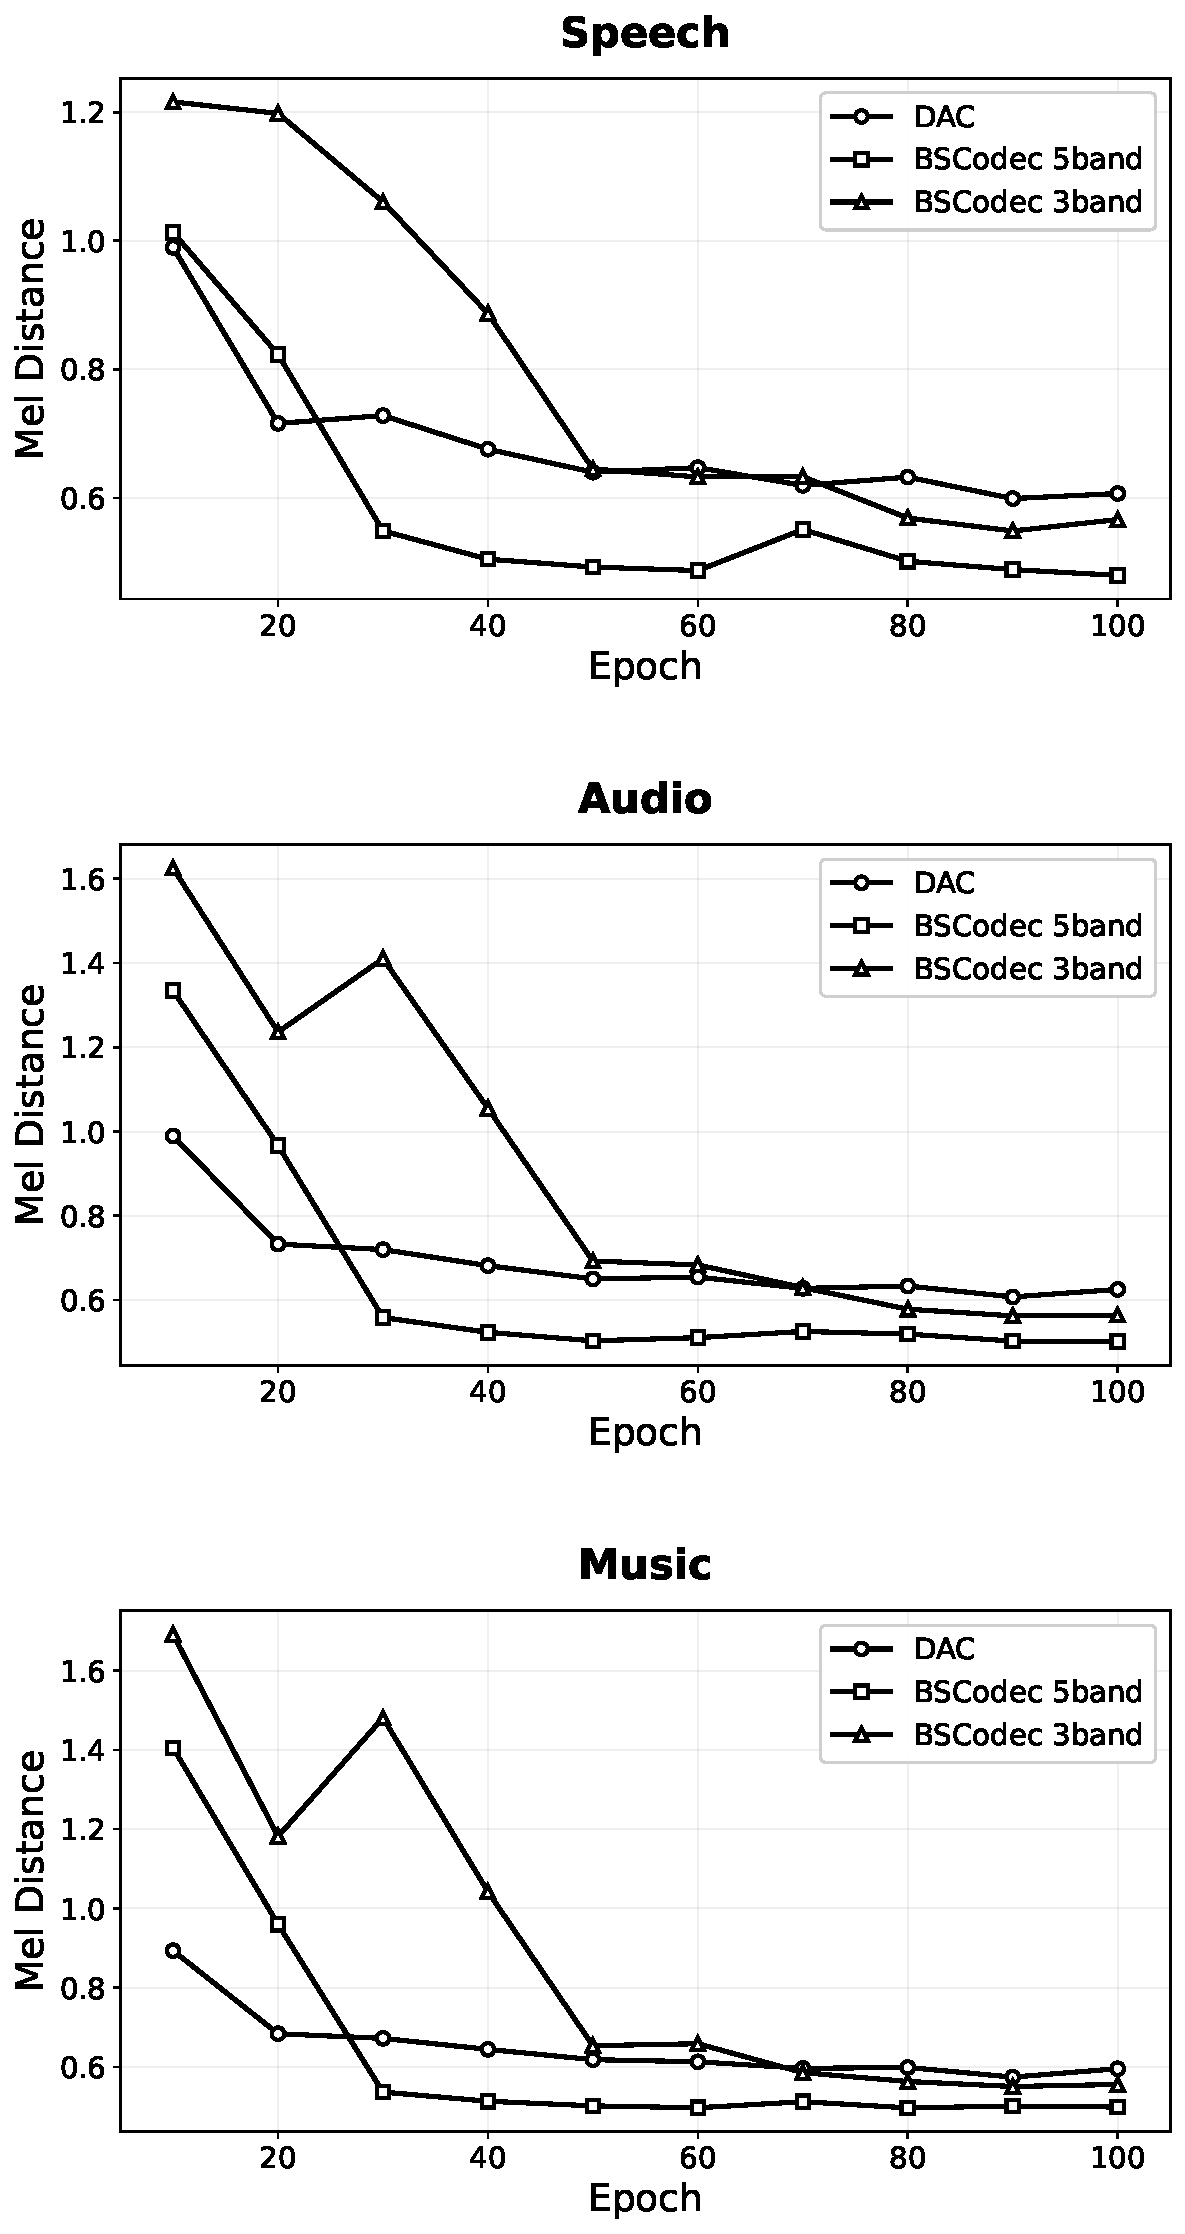
\includegraphics[width=\columnwidth]{pic/codec_mel_distance_final.pdf}
    \caption{Comparison of the decrease in MEL distance during training for different codecs}
    \label{fig:codec_comparison}
\end{figure}

We compare the convergence speed of different codec architectures by tracking Mel Distance throughout training on the three-domain mixed dataset. Evaluations are conducted every 10 epochs, with each epoch processing 2000 samples.

Figure~\ref{fig:codec_comparison} shows the convergence curves across the three domains. DAC exhibits slower convergence with flatter curves across all domains. Both BSCodec 5-band and 3-band configurations reach stable performance within approximately 40-60 epochs, showing steeper descent in the early training phase.

% \section{Single-Domain Training Performance}

% In the main paper, we introduced band splitting on the music domain first, as music exhibits a broad fundamental frequency distribution that naturally motivates frequency decomposition. However, we also conducted experiments training models exclusively on speech and audio domains to evaluate the effectiveness of band partitioning across different acoustic characteristics.

% We train separate models on individual domains using the same training configurations as the multi-domain setup. For speech, we use the LibriTTS dataset; for audio, we use AudioSet; and for music, we use MUSDB. Each model is trained for the same number of iterations and evaluated using domain-appropriate metrics.

% Table~\ref{tab:single_domain} presents the performance comparison between DAC and BSCodec variants when trained on single domains. [Results to be added]



% \section{Codebook Utilization Calculation}
% \label{app:2}

% In traditional multi-layer codebook analysis, utilization is computed by calculating the entropy of each layer independently and comparing it to the theoretical maximum entropy. However, this layer-wise approach fails to capture inter-layer dependencies that are critical for understanding the true capacity usage of multi-layer quantization schemes.

% For a codec with $L$ layers, each having a codebook of size $K$, treating all layers as a single unified codebook yields a theoretical space of size $K^L$. For example, an 8-layer RVQ codec with $K=1024$ per layer corresponds to a joint codebook of size $2^{80}$ (approximately $10^{24}$). Computing the true entropy of such a massive discrete distribution would require statistics over an impractically large audio dataset and is computationally infeasible.

% To measure inter-layer correlation while maintaining computational tractability, we adopt a pairwise analysis approach. Specifically, we compute the joint utilization of consecutive layer pairs, treating each pair as a combined codebook of size $K^2$. For layers $i$ and $i+1$, let $c_i$ and $c_{i+1}$ denote the codebook indices selected for a given frame. The joint distribution is:
% \begin{equation}
% p(c_i, c_{i+1}) = \frac{\text{count}(c_i, c_{i+1})}{N}
% \end{equation}
% where $N$ is the total number of frames in the evaluation dataset. The joint entropy is:
% \begin{equation}
% H(c_i, c_{i+1}) = -\sum_{j=1}^{K} \sum_{k=1}^{K} p(j, k) \log_2 p(j, k)
% \end{equation}

% The pairwise codebook utilization rate is then defined as:
% \begin{equation}
% U_{i,i+1} = \frac{H(c_i, c_{i+1})}{2\log_2 K}
% \end{equation}
% where the denominator $2\log_2 K$ represents the theoretical maximum entropy for two independent uniform distributions over $K$ entries. A utilization rate approaching 1.0 indicates that the two layers are nearly statistically independent and fully utilized, while values significantly below 1.0 suggest redundancy or correlation between layers.

% For RVQ-based codecs, we compute $U_{i,i+1}$ for all consecutive pairs $(i, i+1)$ where $i \in \{1, 2, \ldots, L-1\}$ to assess the degree of independence across the residual hierarchy. 

\section{Codebook Utilization Calculation}
\label{app:2}

For a single-layer codebook with size $K$, the utilization rate is computed by calculating the entropy of the codebook usage distribution and comparing it to the theoretical maximum entropy. Our calculation methodology follows the approach used in DAC~\cite{kumar2023high}. Let $c$ denote the codebook index selected for a given frame, and $p(c)$ be its empirical distribution over the evaluation dataset. The single-layer entropy is:
\begin{equation}
H(c) = -\sum_{j=1}^{K} p(j) \log_2 p(j)
\end{equation}
The single-layer utilization rate is then:
\begin{equation}
U = \frac{H(c)}{\log_2 K}
\end{equation}
where $\log_2 K$ represents the theoretical maximum entropy for a uniform distribution over $K$ entries.

However, this layer-wise approach fails to capture inter-layer dependencies that are critical for understanding the true capacity usage of multi-layer quantization schemes. For a codec with $L$ layers, each having a codebook of size $K$, treating all layers as a single unified codebook yields a theoretical space of size $K^L$. For example, an 8-layer RVQ codec with $K=1024$ per layer corresponds to a joint codebook of size $2^{80}$ (approximately $10^{24}$). Computing the true entropy of such a massive discrete distribution would require statistics over an impractically large audio dataset and is computationally infeasible.

To measure inter-layer correlation while maintaining computational tractability, we adopt a pairwise analysis approach. Specifically, we compute the joint utilization of consecutive layer pairs, treating each pair as a combined codebook of size $K^2$. For layers $i$ and $i+1$, let $c_i$ and $c_{i+1}$ denote the codebook indices selected for a given frame. The joint distribution is:
\begin{equation}
p(c_i, c_{i+1}) = \frac{\text{count}(c_i, c_{i+1})}{N}
\end{equation}
where $N$ is the total number of frames in the evaluation dataset. The joint entropy is:
\begin{equation}
H(c_i, c_{i+1}) = -\sum_{j=1}^{K} \sum_{k=1}^{K} p(j, k) \log_2 p(j, k)
\end{equation}
The pairwise codebook utilization rate is then defined as:
\begin{equation}
U_{i,i+1} = \frac{H(c_i, c_{i+1})}{2\log_2 K}
\end{equation}
where the denominator $2\log_2 K$ represents the theoretical maximum entropy for two independent uniform distributions over $K$ entries. A utilization rate approaching 1.0 indicates that the two layers are nearly statistically independent and fully utilized, while values significantly below 1.0 suggest redundancy or correlation between layers.

For RVQ-based codecs, we compute $U_{i,i+1}$ for all consecutive pairs $(i, i+1)$ where $i \in \{1, 2, \ldots, L-1\}$ to assess the degree of independence across the residual hierarchy.

\section{Speech Reconstruction Metrics}
\label{app:3}
% WB-PESQ STOI UTMOS SPK\_SIM VISQOL 

We provide detailed descriptions of the speech quality metrics used in our evaluation.

\noindent\textbf{Wide-Band Perceptual Evaluation of Speech Quality (WB-PESQ)} is an ITU-T P.862.2 standard metric that predicts subjective listening quality by comparing processed speech to its clean reference. It outputs scores ranging from -0.5 to 4.5, with higher values indicating better perceptual quality.

\noindent\textbf{Short-Time Objective Intelligibility (STOI)} evaluates speech intelligibility by measuring the correlation between short-time temporal envelopes of processed and reference signals. Scores range from 0 to 1, with higher values indicating better intelligibility.

\noindent\textbf{UTMOS (University of Tokyo Mean Opinion Score)} is a deep learning-based metric that predicts the subjective Mean Opinion Score of synthesized speech without human listeners. It provides scores from 1 to 5, where higher scores indicate better perceived quality.

\noindent\textbf{SPK\_SIM (Speaker Similarity)} measures the preservation of speaker characteristics by computing the cosine similarity between speaker embeddings extracted from synthesized and ground-truth utterances using ESPnet-SPK~\cite{jung2024espnet}. Values range from 0 to 1, with higher scores indicating better speaker identity preservation.

\noindent\textbf{VISQOL (Virtual Speech Quality Objective Listener)} is a full-reference metric that predicts perceived audio quality by measuring spectro-temporal similarity between processed and reference signals. Scores range from 1 to 5, with higher values indicating better quality.


\section{Energy Distribution Extraction}
\label{app:energy_extraction}

We extract energy distributions from audio files using the following pipeline:

\noindent\textbf{Preprocessing:} All audio samples are normalized to -23.0 LUFS using pyloudnorm to ensure fair comparison across recordings.

\noindent\textbf{Spectral analysis:} We compute the Short-Time Fourier Transform (STFT) with FFT size $N_{\text{FFT}} = 2048$ and hop length $H = 512$. The energy spectrum is obtained as $E_i(f, t) = |X_i(f, t)|^2$, where $X_i(f, t)$ are the STFT coefficients for file $i$.

\noindent\textbf{Weighted averaging:} For each category (sound, music, speech), we compute the weighted average across all files:
\begin{equation}
    E_{\text{category}}(f) = \frac{\sum_{i=1}^{N} \sum_{t=1}^{T_i} E_i(f, t)}{\sum_{i=1}^{N} T_i}
\end{equation}
where $N$ is the number of files and $T_i$ is the number of frames in file $i$.
The results are plotted on a semi-log scale for 0--8~kHz.


\section{Data Distribution}
\label{app:4}


\begin{table}[htbp]
\centering
\caption{Datasets of Stage 1.}
\label{tab:data_distribution_stage2}
\resizebox{0.48\textwidth}{!}{
\renewcommand{\arraystretch}{1.3}
\begin{tabular}{l c p{6cm}}
\hline
\textbf{Dataset} & \textbf{Duration (hours)} & \textbf{Description} \\
\hline
MTG-Jamendo & 3,764.42 & Open music dataset \\[0.2cm]
MAESTRO & 194.27 & Classical piano performances \newline with aligned MIDI \\[0.2cm]
MUSDB18 & 6.04 & 150 full-length music \newline tracks \\[0.2cm]
\hline
Total & 3,964.73 & \\
\hline
\end{tabular}
}
\end{table}




\begin{table}[h]
\centering
\caption{Datasets of Stage 2.}
\label{tab:data_distribution}
\resizebox{0.48\textwidth}{!}{
\renewcommand{\arraystretch}{1.3}
\begin{tabular}{l c p{6cm}}
\hline
\textbf{Dataset} & \textbf{Duration (hours)} & \textbf{Description} \\
\hline
AudioSet & 742.51 & Large-scale manually \newline annotated audio events \\[0.2cm]
CommonVoice & 14.93 & Multilingual transcribed \newline speech corpus \\[0.2cm]
MTG-Jamendo & 753.82 & Open music dataset \\[0.2cm]
LibriTTS & 528.94 & Multi-speaker English \newline audiobook corpus \\[0.2cm]
MUSDB18 & 6.04 & 150 full-length music \newline tracks \\[0.2cm]
VCTK & 80.80 & 110 English speakers \newline with various accents \\[0.2cm]
\hline
Total & 2,127.04 & \\
\hline
\end{tabular}
}
\end{table}
%为了消除SimVQ本身对实验结果可信度的影响，我们也尝试了用Residual SimVQ，以及将band vq中的VQ改成SimVQ，实验效果见表5。可以看到，无论是将DAC的RVQ换成Residual SimVQ，还是将5band配置下的BScodec的VQ改成SimVQ，并没有给模型的性能带来很大的提升。所以在我们的实验中，SimVQ仅仅作为在大码本上进行量化的工具，而且前面的也给出，SimVQ的码本利用率和DAC实际上是相近的。所以其本身的设计并不是模型取得优秀性能的决定性因素。

% \subsection{Training Objective}

% % 对于loss，我们考虑过这样严格要求每个band的重构目标为这个band的原始音频会不会太过于严苛，因为这等价于每个切分后的窄的频带只需要约1kbps就能够重构。虽然BigCodec已经证明了将编解码器的能力scale到一定程度，可以用单层码本很好的还原音频，但我们这里采取的是比BigCodec小得多的编解码器。所以我们尝试了放宽Loss的限制，对于第n个band，计算loss是选前n的band重构的音频之和和ground truth的前n个band进行比较。理论上这种设计提供了更高的表示上限，但是实验结果表明这种设计的表现会略差于我们提出的设计。所以在我们的设计中，单个码本的容量足以对一个窄带进行编码。
% For the training objective, we investigate whether enforcing each band to strictly reconstruct its corresponding frequency range is overly restrictive, as this essentially requires each narrow frequency band to be reconstructed with approximately 1 kbps. While BigCodec has demonstrated that scaling codec capacity enables high-quality audio reconstruction with a single-layer codebook, our encoder-decoder architecture is considerably smaller than BigCodec. Therefore, we explore a relaxed loss design: for the $n$-th band, we compute the loss by comparing the sum of reconstructed audio from the first $n$ bands against the ground truth sum of the first $n$ bands. Theoretically, this design provides a higher representational capacity upper bound. However, experimental results indicate that this design performs slightly worse than our proposed approach. This suggests that in our design, a single codebook possesses sufficient capacity to encode a narrow frequency band.



% appendix：
% 1. 数据集domain的难度， 2. 收敛时在各个domain上的收敛速度，用通用指标比如mel loss，stft loss之类的。





% \begin{table*}[t]
% \centering
% \caption{Performance comparison on music and instrument domains}
% \label{tab:music_instrument_results}
% \begin{tabular}{lcccccc}
% \toprule
% & \multicolumn{3}{c}{Music} & \multicolumn{3}{c}{Instrument} \\
% \cmidrule(lr){2-4} \cmidrule(lr){5-7}
% Model & VISQOL$\uparrow$ & Mel Dist.$\downarrow$ & STFT Dist.$\downarrow$ & VISQOL$\uparrow$ & Mel Dist.$\downarrow$ & STFT Dist.$\downarrow$ \\
% \midrule
% DAC (6 kbps) & 4.097 & 0.481 & 1.018 & 4.479 & 0.506 & 0.959 \\
% VQ 5-band (3.75 kbps) & \textbf{4.384} & \textbf{0.445} & \textbf{0.921} & 4.470 & 0.419 & 0.788 \\
% SimVQ 5-band (3.75 kbps) & 4.274 & 0.493 & 1.070 & 4.484 & 0.442 & 0.841 \\
% SimVQ 3-band (3.825 kbps) & 4.196 & 0.477 & 1.042 & 4.495 & \textbf{0.412} & \textbf{0.787} \\
% SimVQ 2-band (2.55 kbps) & 4.104 & 0.482 & 0.994 & 4.484 & 0.417 & 0.806 \\
% RSimVQ (4.5 kbps) & 4.106 & 0.475 & 1.039 & \textbf{4.514} & 0.444 & 0.848 \\
% \bottomrule
% \end{tabular}
% \end{table*}


% \begin{table*}[t]
% \centering
% \caption{Performance comparison on speech domain}
% \label{tab:speech_results}
% \begin{tabular}{lcccccc}
% \toprule
% \multicolumn{2}{c}{Model} & \multicolumn{5}{c}{Speech} \\
% \cmidrule(lr){1-2} \cmidrule(lr){3-7}
% Model & Bitrate & MCD$\downarrow$ & PESQ$\uparrow$ & STOI$\uparrow$ & SPK\_SIM$\uparrow$ & UTMOS$\uparrow$ \\
% \midrule
% DAC & 6.00 kbps & 5.40 & \textbf{2.915} & \textbf{0.934} & 0.751 & 3.356 \\
% DAC & 4.50 kbps & - & - & - & - & - \\
% RSimVQ & 4.50 kbps & 6.00 & 2.462 & 0.906 & 0.662 & 2.655 \\
% 5-band VQ & 3.75 kbps & 5.08 & 1.961 & 0.894 & 0.810 & 2.515 \\
% 5-band SimVQ & 3.75 kbps & 5.66 & 2.030 & 0.892 & 0.774 & 2.723 \\
% 3-band SimVQ & 3.83 kbps & \textbf{5.05} & 2.544 & 0.920 & \textbf{0.852} & \textbf{3.360} \\
% 2-band SimVQ & 2.55 kbps & 5.42 & 2.429 & 0.916 & 0.783 & 3.304 \\
% \bottomrule
% \end{tabular}
% \end{table*}

% \begin{table*}[t]
% \centering
% \caption{Performance comparison on audio and music domains}
% \label{tab:audio_music_results}
% \begin{tabular}{lcccccccc}
% \toprule
% \multicolumn{2}{c}{Model} & \multicolumn{3}{c}{Audio} & \multicolumn{3}{c}{Music} \\
% \cmidrule(lr){1-2} \cmidrule(lr){3-5} \cmidrule(lr){6-8}
% Model & Bitrate & VISQOL$\uparrow$ & Mel Dist.$\downarrow$ & STFT Dist.$\downarrow$ & VISQOL$\uparrow$ & Mel Dist.$\downarrow$ & STFT Dist.$\downarrow$ \\
% \midrule
% DAC & 6.00 kbps & 4.085 & \textbf{0.452} & 0.874 & 4.201 & \textbf{0.439} & 0.974 \\
% DAC & 4.50 kbps & - & - & - & - & - & - \\
% RSimVQ & 4.50 kbps & 4.068 & 0.469 & 0.851 & 4.172 & 0.444 & 0.899 \\
% 5-band VQ & 3.75 kbps & \textbf{4.245} & 0.463 & 0.800 & \textbf{4.326} & 0.464 & 0.892 \\
% 5-band SimVQ & 3.75 kbps & 4.185 & 0.476 & 0.814 & 4.267 & 0.476 & 0.903 \\
% 3-band SimVQ & 3.83 kbps & 4.234 & \textbf{0.456} & \textbf{0.794} & 4.298 & 0.461 & \textbf{0.888} \\
% 2-band SimVQ & 2.55 kbps & 4.137 & 0.470 & 0.846 & 4.166 & 0.479 & 0.916 \\
% \bottomrule
% \end{tabular}
% \end{table*}



% \begin{table*}[t]
% \centering
% \caption{Performance comparison on classification tasks}
% \label{tab:classification_results}
% \begin{tabular}{lccccccc}
% \toprule
% & \multicolumn{2}{c}{Speech} & \multicolumn{3}{c}{Audio} & \multicolumn{2}{c}{Music} \\
% \cmidrule(lr){2-3} \cmidrule(lr){4-6} \cmidrule(lr){7-8}
% Model & RAVDESS$\uparrow$ & AM$\uparrow$ & ESC-50$\uparrow$ & US8K$\uparrow$ & VIVAE$\uparrow$ & MTT$\uparrow$ & MS-DB$\uparrow$ \\
% \midrule
% DAC & 0.3958 & 0.7791 & 0.3335 & 0.5311 & \textbf{0.3285} & 0.2949 & 0.5754 \\
% 3-band SimVQ & \textbf{0.4306} & 0.7759 & 0.3725 & 0.5654 & 0.3258 & 0.3531 & 0.6969 \\
% 2-band SimVQ & 0.4201 & \textbf{0.7801} & \textbf{0.3795} & \textbf{0.5798} & 0.3265 & \textbf{0.3555} & \textbf{0.7021} \\
% \bottomrule
% \end{tabular}
% \end{table*}





% \begin{table*}[t]
% \centering
% % 在标题中增加一句来说明粗体的含义
% \caption{Objective evaluation results. We compare our different configurations against the DAC baseline on the music and instrument domains. For ViSQOL, higher is better ($\uparrow$). For Mel Distance and STFT Distance, lower is better ($\downarrow$). The best results in each column are highlighted in \textbf{bold}.}
% \label{tab:objective_results}
% \begin{tabular}{@{}l l c ccc ccc@{}}
% \toprule
% \textbf{Model} & \textbf{Config} & \textbf{Bitrate} & \multicolumn{3}{c}{\textbf{Music}} & \multicolumn{3}{c}{\textbf{Instrument}} \\
% \cmidrule(lr){4-6} \cmidrule(lr){7-9}
% & & (kbps) & ViSQOL $\uparrow$ & Mel Dist. $\downarrow$ & STFT Dist. $\downarrow$ & ViSQOL $\uparrow$ & Mel Dist. $\downarrow$ & STFT Dist. $\downarrow$ \\
% \midrule
% DAC & RVQ & 6 & 4.097 & 0.481 & 1.018 & 4.479 & 0.506 & 0.959 \\
% \midrule
% BScodec & VQ & 3.75 & \textbf{4.304} & \textbf{0.445} & \textbf{0.921} & 4.470 & 0.419 & 0.788 \\
% BScodec & SimVQ & 3.825 & 4.196 & 0.477 & 1.042 & \textbf{4.495} & \textbf{0.412} & \textbf{0.787} \\
% BScodec & SimVQ & 2.55 & 4.104 & 0.482 & 0.994 & 4.484 & 0.417 & 0.806 \\
% \bottomrule
% \end{tabular}
% \end{table*}


% \begin{table*}[t]
% \centering

% \caption{Speech reconstruction quality evaluation. All models are compared on a speech dataset. For all metrics (MOD, PESQ, STOI, SPK\_SIM), higher scores indicate better performance ($\uparrow$). The best result in each column is highlighted in \textbf{bold}.}
% \label{tab:speech_results}

% \begin{tabular}{@{}l l c cccc@{}}
% \toprule
% \textbf{Model} & \textbf{Config} & \textbf{Bitrate} & \multicolumn{4}{c}{\textbf{Speech}} \\

% \cmidrule(lr){4-7}
% & & (kbps) & MCD $\downarrow$ & PESQ $\uparrow$ & STOI $\uparrow$ & SPK\_SIM $\uparrow$ \\
% \midrule
% DAC & RVQ & 6 & 5.78 & \textbf{2.842} & \textbf{0.923} & 0.647 \\
% \midrule
% BScodec & VQ & 3.75 & 5.72 & 1.960 & 0.883 & 0.749 \\
% BScodec & SimVQ & 3.825 & \textbf{5.73} & 2.627 & 0.914 & \textbf{0.815} \\
% BScodec & SimVQ & 2.55 & 6.24 & 2.362 & 0.887 & 0.694 \\
% \bottomrule
% \end{tabular}
% \end{table*}


% \begin{table*}[t]
% \centering

% \caption{Objective evaluation on general audio and music datasets. We compare our configurations against the DAC baseline. For ViSQOL, higher is better ($\uparrow$), while for Mel/STFT Distance, lower is better ($\downarrow$). The best result in each column is highlighted in \textbf{bold}.}
% \label{tab:audio_music_results}

% \begin{tabular}{@{}l l c ccc ccc@{}}
% \toprule
% \textbf{Model} & \textbf{Config} & \textbf{Bitrate} & \multicolumn{3}{c}{\textbf{Audio}} & \multicolumn{3}{c}{\textbf{Music}} \\

% \cmidrule(lr){4-6} \cmidrule(lr){7-9}
% & & (kbps) & ViSQOL $\uparrow$ & Mel Dist. $\downarrow$ & STFT Dist. $\downarrow$ & ViSQOL $\uparrow$ & Mel Dist. $\downarrow$ & STFT Dist. $\downarrow$ \\
% \midrule
% DAC & RVQ & 6 & 4.006 & 0.471 & 0.907 & 4.182 & \textbf{0.450} & 0.977 \\
% \midrule
% BScodec & VQ & 3.75 & 4.161 & 0.475 & 0.832 & 4.254 & 0.462 & 0.898 \\
% BScodec & SimVQ & 3.825 & \textbf{4.247} & \textbf{0.469} & \textbf{0.810} & \textbf{4.298} & 0.462 & \textbf{0.890} \\
% BScodec & SimVQ & 2.55 & 4.091 & 0.488 & 0.846 & 4.166 & 0.479 & 0.916 \\
% \bottomrule
% \end{tabular}
% \end{table*}


% Bibliography entries for the entire Anthology, followed by custom entries
% \bibliography{anthology,custom}
% Custom bibliography entries only


% \appendix

% \section{Example Appendix}
% \label{sec:appendix}

% This is an appendix.

\end{document}
